\documentclass[article, 12pt, 3p]{elsarticle}

\usepackage{natbib} 
\setcitestyle{authoryear,open={(},close={)}}
%\bibliographystyle{plainnat}

\usepackage{etoolbox,comment,setspace,fancyhdr,hyperref,color,graphicx,subcaption,booktabs,rotating,multirow}

\captionsetup[subfigure]{labelformat=simple,labelsep=space}
\renewcommand\thesubfigure{(\roman{subfigure})}

\newcounter{rowfig}
\renewcommand{\therowfig}{\Alph{rowfig}}

\usepackage{amsmath,amsthm,amssymb,amstext,bbold,amsfonts}
\usepackage{float,caption}
\usepackage{threeparttable}
\usepackage{lscape}
\usepackage{bbm}
\usepackage{adjustbox}
\usepackage[tracking=true]{microtype}
%\usepackage[pdftex, letterpaper, margin=1in, headheight=-.25cm]{geometry}
 %\usepackage[abbr]{harvard}
 
\hypersetup{
  colorlinks   = true, %Colours links instead of ug dly boxes
  urlcolor     = blue, %Colour for external hyperlinks
  linkcolor    = black, %Colour of internal links 
  citecolor   = blue %Colour of citations
}

\newtheorem{proposition}{Proposition}
\newtheorem{definition}{Definition}
\newtheorem{assumption}{Assumption}
\newtheorem{condition}{Condition}
\newtheorem{lemma}{Lemma}
\newtheorem{conjecture}{Conjecture}
\newtheorem{corollary}{Corollary}
\numberwithin{corollary}{proposition}
%\numberwithin{equation}{section}
% [[prompt01]] original: \numberwithin{equation}{}

%\newcommand{\inv}{\makebox[0pt][l]{$^{-1}$}}
\pdfoptionpdfminorversion=6 

%Define argmax
\DeclareMathOperator*{\argmax}{arg\,max}

%%Put space between captions and figures.
%\setlength{\belowcaptionskip}{6pt}

\makeatletter
\def\ps@pprintTitle{%
   \let\@oddhead\@empty
   \let\@evenhead\@empty
   \let\@oddfoot\@empty
   \let\@evenfoot\@oddfoot
}
\makeatother
\usepackage{ragged2e}
\usepackage{setspace} 
\usepackage{caption}
% [[prompt01]] original: \usepackage[usenames,dvipsnames]{pstricks}
% [[prompt01]] original: \usepackage{epsfig}
% [[prompt01]] original: \usepackage{pst-grad} % For gradients
% [[prompt01]] original: \usepackage{pst-plot} % For axes
 \usepackage[space]{grffile} % For spaces in paths
 \makeatletter % For spaces in paths
 \patchcmd\Gread@eps{\@inputcheck#1 }{\@inputcheck"#1"\relax}{}{}
 \makeatother
\usepackage[utf8]{inputenc}
% [[prompt01]] original: \usepackage{stackrel}
\IfFileExists{stackrel.sty}{\usepackage{stackrel}}{}
\usepackage{array}
\usepackage{siunitx}
% [[prompt02]] added: column-width convention of the reference (_reference_productivity/Tables/_tabledefs.tex,
% copied, not \input): N{<width>} centred numeric column, L{<width>} ragged-right label column.
\usepackage{makecell}
\newcolumntype{N}[1]{>{\centering\arraybackslash}p{#1}}
\newcolumntype{L}[1]{>{\raggedright\arraybackslash}p{#1}}
\newlength{\labelw}\setlength{\labelw}{0.22\textwidth}
\newlength{\labelwwide}\setlength{\labelwwide}{0.36\textwidth}
\newlength{\labelwnarrow}\setlength{\labelwnarrow}{0.19\textwidth}
\newcommand{\colwfor}[2]{\dimexpr(\textwidth-(#2)-\tabcolsep*\numexpr2*#1+2\relax)/#1\relax}
\newcommand{\colwform}[3]{\dimexpr(\textwidth-(#3)-\tabcolsep*\numexpr2*#1+2*#2\relax)/#1\relax}
\newcommand{\colw}{\colwfor{6}{\labelw}}
\newcommand{\colwvii}{\colwfor{7}{\labelw}}
\newcommand{\colwnarrow}{\colwfor{8}{\labelw}}
\newcommand{\notesize}{\footnotesize}
\setlength{\extrarowheight}{4pt}
\renewcommand\normalsize{\fontsize{11}{8}\selectfont}
\newcommand\narrowstyle{\SetTracking{encoding=*}{-10}\lsstyle}
\newcommand\vnarrowstyle{\SetTracking{encoding=*}{-40}\lsstyle}
\newcommand\vvnarrowstyle{\SetTracking{encoding=*}{-75}\lsstyle}

\newcommand\narrowtext[1]{\textls[-10]{#1}}
\newcommand\vnarrowtext[1]{\textls[-40]{#1}}
\newcommand\vvnarrowtext[1]{\textls[-75]{#1}}

\makeatletter
\renewcommand\footnotesize{%
   \@setfontsize\footnotesize\@ixpt{9}%
   \abovedisplayskip 8\p@ \@plus2\p@ \@minus4\p@
   \abovedisplayshortskip \z@ \@plus\p@
   \belowdisplayshortskip 4\p@ \@plus2\p@ \@minus2\p@
   \def\@listi{\leftmargin\leftmargini
               \topsep 4\p@ \@plus2\p@ \@minus2\p@
               \parsep 2\p@ \@plus\p@ \@minus\p@
               \itemsep \parsep}%
   \belowdisplayskip \abovedisplayskip
}
\makeatother

\usepackage{setspace}
\usepackage[T1]{fontenc}
\usepackage{lmodern}  % [[v3]] scalable fonts, needed by microtype outside Overleaf
\usepackage{array}
\usepackage{longtable}
\usepackage{pdfpages}
\usepackage{dsfont}
\newcommand{\bc}{\begin{center}}
\newcommand{\ec}{\end{center}}
\newcommand{\bt}{\begin{tabular}}
\newcommand{\et}{\end{tabular}}
\newcommand{\bi}{\begin{itemize}}
\newcommand{\ei}{\end{itemize}}
\newcommand{\ben}{\begin{enumerate}}
\newcommand{\een}{\end{enumerate}}
\newcommand{\bd}{\begin{displaymath}}
\newcommand{\ed}{\end{displaymath}}
\newcommand{\beann}{\begin{eqnarray*}}
\newcommand{\eeann}{\end{eqnarray*}}
\newcommand{\bea}{\begin{eqnarray}}
\newcommand{\eea}{\end{eqnarray}}
\newcommand{\ba}{\begin{array}}
\newcommand{\ea}{\end{array}}
\newcommand{\bma}{\begin{pmatrix}}
\newcommand{\ema}{\end{pmatrix}}
%}}}
%Math Shortcuts {{{
\newcommand{\Ra}{\Rightarrow}
\newcommand{\bbR}{\mathbb{R}}
\newcommand{\bbY}{\mathbb{Y}}
\newcommand{\bbF}{\mathbb{F}}
\newcommand{\bbS}{\mathbb{S}}
\newcommand{\bbN}{\mathbb{N}}
\newcommand{\bbG}{\mathbb{G}}
\newcommand{\bbT}{\mathbb{T}}
\newcommand{\deB}{\mathcal{B}}
\newcommand{\deW}{\mathcal{W}}
\newcommand{\deR}{\mathcal{R}}
\newcommand{\deF}{\mathcal{F}}
\newcommand{\deA}{\mathcal{A}}
\newcommand{\deY}{\mathcal{Y}}
\newcommand{\deS}{\mathcal{S}}
\newcommand{\deL}{\mathcal{L}}
\newcommand{\deH}{\mathcal{H}}
\newcommand{\deE}{\mathcal{E}}
\newcommand{\deP}{\mathcal{P}}
\newcommand{\deG}{\mathcal{G}}
\newcommand{\deT}{\mathcal{T}}
\newcommand{\deff}{\mathcal{f}}
\newcommand{\dep}{\mathcal{p}}
\newcommand{\E}{\mathnormal{E}}
\newcommand{\var}{\mathnormal{V\!AR}}
\newcommand{\Cov}{\mathnormal{COV}}
\newcommand{\Corr}{\mathnormal{CORR}}
\newcommand{\Prob}{\mathnormal{Prob}}
%}}}
%Additional Shortcuts {{{
\newcommand{\mD}{\displaystyle}
\newcommand{\mT}{\textstyle}
\newcommand{\mS}{\scriptstyle}
\newcommand{\mSS}{\scriptscriptstyle}
\newcommand{\m}[1]{\,#1\,}
\newcommand{\nn}{\nonumber}
\newcommand{\colorEmphText}{\color{blue}}
\newcommand{\colorEmphBackground}{\color{yellow}}
%}}}
% \usepackage[stable]{footmisc} 
\newcommand*{\mycommand}[1]{\texttt{\emph{#1}}}
% [[prompt01]] original: \renewcommand*{\thefootnote}{\fnsymbol{footnote}}
%% these three are essential for estout
\usepackage{booktabs}  % neatly formatting lines
\usepackage{threeparttable}    
\usepackage{dcolumn}    % aligning decimals
    \newcolumntype{d}[1]{D{.}{.}{#1}}
% Estout LaTeX wrapper (by Jörg Weber)
\let\estinput=\input % define a new input command so that we can still flatten the document
\newcommand{\estwide}[3]{
		\vspace{.75ex}{
			%\textsymbols% Note the added command here
			\begin{tabular*}
			{\textwidth}{@{\hskip\tabcolsep\extracolsep\fill}l*{#2}{#3}}
			\toprule
			\estinput{#1}
			\addlinespace[.75ex]
			\end{tabular*}
			}
		}	
\newcommand{\estauto}[3]{
		\vspace{.75ex}{
			%\textsymbols% Note the added command here
			\begin{tabular}{l*{#2}{#3}}
			\toprule
			\estinput{#1}
			\\ \bottomrule           % 08 Dec 2021. Add these slashes.
			\addlinespace[-.75]
			\end{tabular}
			}
		}
% Allow line breaks with \\ in specialcells
\newcommand{\specialcell}[2][c]{%
    \begin{tabular}[#1]{@{}c@{}}#2\end{tabular}
}
\usepackage{float}
\usepackage[section]{placeins}
% [[prompt02d]] floats share pages with text instead of going to float pages
\renewcommand{\topfraction}{0.9}
\renewcommand{\bottomfraction}{0.8}
\renewcommand{\textfraction}{0.07}
\renewcommand{\floatpagefraction}{0.85}
\setcounter{topnumber}{3}
\setcounter{bottomnumber}{2}
\setcounter{totalnumber}{4}
\setlength{\floatsep}{10pt plus 2pt minus 2pt}
\setlength{\textfloatsep}{14pt plus 2pt minus 2pt}
\setlength{\intextsep}{12pt plus 2pt minus 2pt}
\newcommand{\sym}[1]{\rlap{#1}}% Thanks David Carlisle
\usepackage{hhline}
\captionsetup{font=normalsize} 


 % Note/Source/Text after Tables
\newcommand{\figtext}[1]{
	\vspace{-1.9ex}
	\captionsetup{justification=justified,font=scriptsize}
	\caption*{\hspace{6pt}\hangindent=1.5em #1}
	} 
\newcommand{\fignote}[1]{\figtext{\emph{Note:~}~#1}}

\newcommand{\figsource}[1]{\figtext{\emph{Source:~}~#1}}

% Add significance note with \starnote
\newcommand{\starnote}{\figtext{* p < 0.1, ** p < 0.05, *** p < 0.01. Standard errors in parentheses.}}
% [[prompt01]] added: source note of every table and figure (wording from main.tex l. 16)
% [[prompt02]] original: \newcommand{\srcnote}{\textit{Source:} Authors' calculations based on customs data matched to Orbis and Dun \& Bradstreet.}
\newcommand{\srcnote}{\textit{Source:} Authors' calculations based on customs data matched to Orbis (Bureau van Dijk) and Dun \& Bradstreet.}
%\usepackage{etoolbox} % to hook into `figure` and reset the mysubfig counter

% [[prompt01]] original: \usepackage{subfig}


% Checkmarks
\usepackage{tikz}
\newcommand{\tikzxmark}{%
\tikz[scale=0.23] {
    \draw[line width=0.7,line cap=round] (0,0) to [bend left=6] (1,1);
    \draw[line width=0.7,line cap=round] (0.2,0.95) to [bend right=3] (0.8,0.05);
}}
\newcommand{\tikzcmark}{% 
\tikz[scale=0.23] {
    \draw[line width=0.7,line cap=round] (0.25,0) to [bend left=10] (1,1);
    \draw[line width=0.8,line cap=round] (0,0.35) to [bend right=1] (0.23,0);
}}
%\renewcommand{\arraystretch}{0.9}
% [[prompt02]] original: \renewcommand{\arraystretch}{0.8}
% [[prompt02]] original: \setlength{\tabcolsep}{5pt}
 \makeatletter
\newcommand*\mysize{%
  \@setfontsize\mysize{7.5}{9.0}%
}

\makeatother
% For reference:
%\[
%    \checkmark
%    \tikzxmark
%    \tikzcmark
%\]

%\onehalfspacing

% [[prompt03b]] elsarticle draws two rules around the (absent) abstract; suppress them for this summary
\makeatletter
\let\els@maketitle\maketitle
\renewcommand{\maketitle}{\begingroup\let\hrule\relax\els@maketitle\endgroup}
\makeatother
\usepackage{pgfplots}\pgfplotsset{compat=1.16}  % [[v3]] figures drawn in the note itself
\hyphenpenalty=10000 \exhyphenpenalty=10000  % [[v3]] no words split across lines with a hyphen

% [[v4]] float macros: label, caption, content, notes, source
\newcommand{\SIG}{*** $p<0.01$, ** $p<0.05$, * $p<0.1$.}
\newcommand{\vtab}[5]{\begin{table}[htbp]\centering\caption{#2}\label{#1}
{\footnotesize\setlength{\tabcolsep}{4pt}\setlength{\extrarowheight}{1pt}\adjustbox{max width=\linewidth}{#3}}\par
\begin{minipage}{0.95\linewidth}\notesize\vspace{0.6em}\textit{Notes:} #4\\#5\end{minipage}\end{table}}
\newcommand{\vfig}[5]{\begin{figure}[htbp]\centering\caption{#2}\label{#1}
\adjustbox{max width=\linewidth}{#3}\par
\begin{minipage}{0.9\linewidth}\notesize\vspace{0.6em}\textit{Notes:} #4\\#5\end{minipage}\end{figure}}
\begin{document}

\title{$\,$\\ $\,$\\ $\,$\\\vspace{-4.9em}\LARGE\textbf{Multinational Firms and Agricultural Trade in Latin America}\footnote{The views and interpretations in this paper are strictly those of the authors and should not be attributed to the Inter-American Development Bank, its executive directors, or its member countries.}}
\author{\vskip 2em This version: November 2026\\[2pt] \small Preliminary draft, please do not circulate}

\thispagestyle{empty}
\maketitle
\begin{center}
\begin{minipage}{0.86\linewidth}
\small
\textit{Abstract.} We use firm level customs data from nine Latin American countries, linked to ownership data, to
examine the role of multinational firms in agricultural exports. We show that multinationals ship 47 percent of these
exports, less than in mining and manufacturing, and that a few parent countries and a few large groups account for most
of them. We also find that exports are larger where more multinationals export the same product to the same
destination, and that this association is stronger for farm products with high capital intensity. Finally, we show that
multinationals are not more likely to export capital intensive products and that fewer markets keep local exports after
the first multinational enters, although local exports were already growing before entry.\\[4pt]
\textit{JEL codes:} F14, F23, Q17. \textit{Keywords:} multinational firms, agricultural exports, capital intensity, Latin America.
\end{minipage}
\end{center}
\setcounter{page}{0}\setcounter{footnote}{0}
\renewcommand\normalsize{\fontsize{12}{20}\selectfont}\normalsize
\newpage

\section{Introduction}\label{sec:intro}

Agriculture is a major source of export revenue in Latin America. It accounts for 35 percent of the merchandise exports
of the nine countries studied here, and for more than half in Argentina, Paraguay and Uruguay. A small number of large
firms handle much of world agricultural trade. Four trading companies account for most of the world grain trade
(Murphy, Burch and Clapp, 2012, and Clapp, 2015), and multinational firms lead the processing, trading and retail stages
of agricultural value chains (UNCTAD, 2009, and Reardon et al., 2009). However, there is little systematic evidence on
how much of the agricultural exports of the region is shipped by multinational firms and on how their presence relates
to the exports of other firms.

In this paper, we address these questions. More precisely, we ask how large the role of multinationals is in
agricultural exports and who owns them, whether exports are larger where more multinationals are present, and whether
this association differs across products. We organize the analysis around the capital intensity of the product.
Agricultural products differ widely in the machinery and equipment used per worker, from fruit orchards to grain farms
and from fruit packing to oilseed crushing. Firms with better access to capital and technology may have an advantage
in the products that need more of them.

To explore these questions, we use firm level customs data from Argentina, Chile, Colombia, Costa Rica, the Dominican
Republic, El Salvador, Paraguay, Peru and Uruguay over the period 2012 to 2018. We link the exporters to ownership data
from Orbis and Dun \& Bradstreet, which tell us whether an exporter belongs to a multinational group and where its
parent is located. We measure the capital intensity of each product with US census data.

Our main results can be summarized as follows. First, multinationals ship 47 percent of agricultural exports, less than
in mining and fuels (80 percent) or manufacturing (58 percent). Their parents are concentrated in a few countries, and
the twenty largest groups ship half of the exports of foreign affiliates. Second, exports are larger where more
multinationals export the same product to the same destination. A 10 percent increase in the number of multinationals
is associated with exports about 8 percent larger when we compare the same origin, destination and product over time.
Third, this association is stronger for farm products with high capital intensity, mainly grains and oilseeds. Among
processed products we find no robust difference. Fourth, multinationals are not more likely to export capital intensive
products. Fifth, after the first multinational starts to export a product, fewer markets keep local exports, but local
exports were already growing before entry, so these estimates cannot be read as effects.

Our paper contributes to the literature on the export spillovers of foreign firms (Aitken, Hanson and Harrison, 1997)
and on the links between multinationals and local firms (Javorcik, 2004). These studies focus on manufacturing. We
provide evidence for agriculture, where the technology of production varies widely across products. Closer to our
paper, Carballo, Marra de Arti\~nano, Ottaviano and Volpe Martincus (2021) show that domestic firms that start selling
to a multinational are more likely to start exporting, and Carballo, Marra de Arti\~nano and Volpe Martincus (2026) show
that investment promotion raises the probability that a multinational opens its first affiliate in a country. We
complement these studies with evidence on the weight of multinationals in agricultural exports and on how it varies
with the capital intensity of the product. Our estimates describe associations, not causal effects.

The rest of the paper is organized as follows. Section~\ref{sec:data} describes the data. Section~\ref{sec:desc}
documents the weight of multinationals in agricultural exports. Section~\ref{sec:regs} relates their presence to
exports and to capital intensity. Section~\ref{sec:conclusions} concludes.

\section{Data}\label{sec:data}

Our dataset consists of three main databases. First, we have firm level export data from the customs agencies of the
nine countries. The data cover 2012 to 2018, the years in which all nine countries are observed. Each record includes
the tax identifier of the firm, the product code at six digits of the Harmonized System (HS), the destination country,
the year and the export value in US dollars.\footnote{The countries report HS 2007, HS 2012 or HS 2017, depending on the
country and the year. We convert all codes to HS 2017 with the correlation tables of the United Nations Statistics
Division (UNSD, 2026). In the records of Uruguay for 2016 to 2018, the codes of chapters 01 to 09 lost their first digit,
a zero, and we restore it. Destinations are countries. Free trade zones and shipments to the exporting country are
dropped.} Agricultural products are HS chapters 01 to 24. Second, we have data on the global ultimate owner of each
company and the country of that owner from Orbis (Bureau van Dijk) and Dun \& Bradstreet.\footnote{Exporters are linked
to these records by tax identifiers, by name matching confirmed with a large language model, and by a manual review of
the largest unmatched exporters. In 2018, the country of the owner is known for 88 percent of the agricultural exports
of foreign affiliates.} Finally, we measure the capital intensity of the industry behind each product with US data: the
2017 Census of Agriculture (USDA NASS, 2019) for farm products and the Manufacturing Industry Database of the National
Bureau of Economic Research and the Center for Economic Studies (NBER and CES, see Becker, Gray and Marvakov, 2021) for
processed products.

An exporter linked to the ownership data is an affiliate of a multinational firm (MNE), and its ultimate owner is its
parent. The affiliate is a domestic MNE when its parent is located in the exporting country and a foreign MNE
otherwise, including affiliates whose parent country is not recorded. Exporters that cannot be linked are local firms.
A multinational group is the set of affiliates with the same parent. A snapshot of our dataset is presented in
Table~\ref{tab:sample}. In 2018, 13,077 firms exported 782 agricultural products to 211 countries, for a total of
US\$79.4 billion.

\vtab{tab:sample}{Agricultural exports, by exporting country, 2018}{\begin{tabular}{lrrrrr}
\toprule
Country & Exporters & Products & Destinations & Exports (US\$ billion) & Agriculture in total exports (\%) \\
\midrule
Argentina & 2,879 & 473 & 176 & 34.6 & 56.3 \\
Peru & 2,538 & 450 & 146 & 10.0 & 20.9 \\
Chile & 1,542 & 452 & 164 & 8.5 & 24.1 \\
Colombia & 2,413 & 447 & 166 & 7.2 & 17.3 \\
Paraguay & 358 & 171 & 113 & 6.6 & 83.8 \\
Costa Rica & 1,123 & 438 & 127 & 4.8 & 42.5 \\
Uruguay & 471 & 303 & 136 & 4.5 & 66.1 \\
Dominican Republic & 1,320 & 478 & 124 & 2.2 & 23.4 \\
El Salvador & 433 & 342 & 82 & 1.1 & 18.8 \\
\midrule
LAC9 & 13,077 & 782 & 211 & 79.4 & 34.9 \\
\bottomrule
\end{tabular}}
{The table reports agricultural exports, exporters, products and destinations in 2018. Exporters are distinct tax
identifiers within each country. Destinations are countries, without free trade zones and shipments to the exporting
country. LAC9: the nine countries together.}{\srcnote}

Capital intensity is machinery and equipment per hired worker for farm products, from the fourteen farm types of the
census, and equipment capital per employee for processed products, averaged over 2012 to 2018.\footnote{We link HS
products to industries with the UNSD correspondence tables, from HS 2017 to the Central Product Classification, to the
International Standard Industrial Classification and to the North American Industry Classification System 2017. When a
product reaches several farm types or industries, we add up their capital and their workers. The census does not cover
fishing, so fresh fish takes the values of the farm types linked to it, mainly aquaculture.} The measure covers 99
percent of agricultural exports. The products it does not cover, such as bran and ethyl alcohol, are not classified.
Within each stage, a product has high capital intensity when its capital per worker is above that of the stage as a
whole, US\$113 thousand per hired worker on farms and US\$118 thousand per employee in processing. As an alternative,
we use the median of the stage weighted by exports, US\$134 and US\$159 thousand, and quintiles of capital per worker
within each stage. We use the US data only to rank products. We also group products by type of production, based on the
crop groups of the FAO Indicative Crop Classification (FAO, 2015): field crops, horticultural and plantation crops,
livestock and fisheries, and other processed food and beverages.

\section{Multinationals in Agricultural Exports}\label{sec:desc}

In this section, we document how much of the agricultural exports of the region is shipped by multinationals, where
their parents are located and how concentrated their exports are across groups.

\subsection{Multinationals ship almost half of agricultural exports, less than in other sectors}\label{sec:share}

Table~\ref{tab:sector} compares agriculture with the other sectors. When looking at the nine countries together,
multinationals account for 47.2 percent of agricultural exports in 2018, 39.3 percent through foreign affiliates and 7.9
percent through domestic ones. Their weight is larger in mining and fuels, 79.8 percent, and in manufacturing, 58.0
percent. Thus, agriculture is 35.0 percent of the exports of the region but only 27.5 percent of the exports of
multinationals. This hides some variation across countries. The multinational share of agricultural exports ranges
from 30.4 percent in El Salvador to 69.4 percent in Paraguay, and it is lower than in manufacturing in seven of the nine
countries. Paraguay and Peru are the exceptions.

\vtab{tab:sector}{Exports and multinational shares by sector, 2018}{\begin{tabular}{lrrrrrrrr}
\toprule
 & \multicolumn{3}{c}{Exports (US\$ billion)} & \multicolumn{5}{c}{MNE share of exports (\%)} \\
\cmidrule(lr){2-4}\cmidrule(lr){5-9}
Country & Agriculture & Mining and fuels & Manufacturing & Agriculture & Mining and fuels & Fuels & Manufacturing & All goods \\
\midrule
Argentina & 34.6 & 3.8 & 23.1 & 45.2 & 68.2 & 66.3 & 66.1 & 54.5 \\
Peru & 10.0 & 22.3 & 15.5 & 39.9 & 68.1 & 48.9 & 32.7 & 50.7 \\
Chile & 8.5 & 10.5 & 16.0 & 48.7 & 82.9 & 25.7 & 55.0 & 61.8 \\
Colombia & 7.2 & 24.4 & 10.0 & 39.6 & 91.6 & 91.6 & 64.5 & 76.0 \\
Paraguay & 6.6 & 0.1 & 1.2 & 69.4 & 2.1 & 0.1 & 45.5 & 65.2 \\
Uruguay & 4.5 & 0.1 & 2.2 & 61.0 & 10.2 & 0.0 & 65.8 & 61.8 \\
Costa Rica & 4.8 & 0.0 & 6.4 & 46.7 & 92.9 & 35.0 & 68.9 & 59.6 \\
Dominican Republic & 2.2 & 0.2 & 7.0 & 44.6 & 78.5 & 69.3 & 78.6 & 70.6 \\
El Salvador & 1.1 & 0.1 & 4.7 & 30.4 & 79.4 & 93.1 & 52.2 & 48.4 \\
\midrule
LAC9 & 79.4 & 61.4 & 86.0 & 47.2 & 79.8 & 82.7 & 58.0 & 60.1 \\
\bottomrule
\end{tabular}}
{The table reports exports and the share shipped by multinationals in each sector in 2018. Agriculture: HS chapters 01
to 24. Mining and fuels: HS 25 to 27. Fuels: HS 27. Manufacturing: HS 28 to 97. MNE share: percent of the exports of
each sector shipped by foreign and domestic MNEs. LAC9: the nine countries together.}{\srcnote}

Table~\ref{tab:mne} describes the exporters. The 3,218 affiliates that export agricultural products belong to 1,926
groups whose parents are based in 112 countries. Affiliates are a quarter of agricultural exporters, but they are larger
and sell to more markets. On average, a foreign affiliate exported US\$11.9 million and a domestic affiliate US\$10.4
million, against US\$4.3 million for a local firm. They reached 5.5 and 6.1 destinations, against 3.9 for local firms.

\vtab{tab:mne}{Multinationals in agricultural exports, 2018}{\begin{tabular}{lrrrr}
\toprule
 & All exporters & Foreign MNEs & Domestic MNEs & Local firms \\
\midrule
Exports (US\$ billion) & 79.4 & 31.2 & 6.3 & 42.0 \\
Share of exports (\%) & 100.0 & 39.3 & 7.9 & 52.8 \\
Exporters & 13,077 & 2,618 & 600 & 9,859 \\
Exports per exporter (US\$ million) & 6.1 & 11.9 & 10.4 & 4.3 \\
Destinations per exporter & 4.3 & 5.5 & 6.1 & 3.9 \\
Products per exporter & 3.2 & 3.4 & 2.9 & 3.1 \\
\bottomrule
\end{tabular}}
{The table reports the number of exporters of each type and their average exports, destinations and products in 2018.}{\srcnote}

\FloatBarrier
\subsection{Parents are concentrated in a few countries}\label{sec:parents}

Figure~\ref{fig:parents} shows the parent countries of foreign affiliates. Two countries account for more than a third
of the agricultural exports of foreign affiliates with a recorded parent: the United States (23.4 percent) and the
Netherlands (11.6 percent). A further 26.1 percent comes from groups whose parent is registered in jurisdictions such
as Switzerland, Liechtenstein, Luxembourg, Panama and Bermuda. Groups often hold their affiliates through companies
located there, so these countries show where the group is registered rather than where it operates. We therefore
measure concentration both with all recorded parents and with the countries of operation only (Table~\ref{tab:pconc}).
Among the countries of operation, the United States ships 31.7 percent of these exports and the five largest countries
64.9 percent. The Herfindahl index is 1,427, the concentration of seven countries of equal size. Notice that the
Netherlands also hosts holding companies, so part of its share may also reflect registration.

\vfig{fig:parents}{Agricultural exports of foreign multinationals, by parent country, 2018}{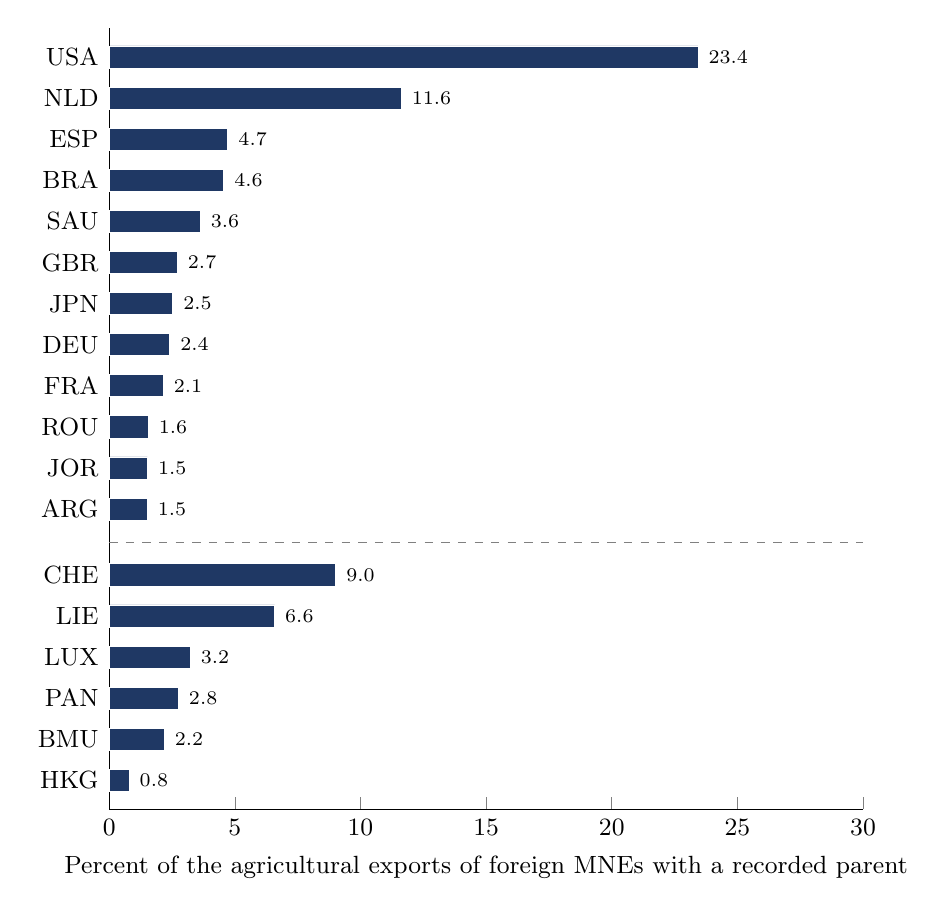
\begin{tikzpicture}
\begin{axis}[
  xbar stacked, bar width=8pt, y dir=reverse,
  width=0.92\linewidth, height=11.5cm, xmin=0, xmax=0.30, ymin=0.30000000000000004, ymax=19.3,
  ytick={1,2,3,4,5,6,7,8,9,10,11,12,13.6,14.6,15.6,16.6,17.6,18.6}, yticklabels={{USA},{NLD},{ESP},{BRA},{SAU},{GBR},{JPN},{DEU},{FRA},{ROU},{JOR},{ARG},{CHE},{LIE},{LUX},{PAN},{BMU},{HKG}},
  xtick={0,0.05,0.1,0.15,0.2,0.25,0.3}, xticklabels={0,5,10,15,20,25,30},
  tick label style={font=\footnotesize}, xlabel={Percent of the agricultural exports of foreign MNEs with a recorded parent}, xlabel style={font=\footnotesize},
  axis x line*=bottom, axis y line*=left, ytick style={draw=none},
  area legend, legend image post style={draw=none}, legend cell align=left, legend style={at={(0.5,0)}, anchor=north, yshift=-1.25cm, draw=none, font=\footnotesize, legend columns=2, /tikz/every even column/.append style={column sep=6pt}}]
\addplot[fill={rgb,255:red,31;green,56;blue,100}, draw=white, line width=0.3pt] coordinates {(0.2343,1) (0.1162,2) (0.0472,3) (0.0456,4) (0.0362,5) (0.0271,6) (0.0253,7) (0.0241,8) (0.0215,9) (0.0155,10) (0.0152,11) (0.0151,12) (0.0901,13.6) (0.0658,14.6) (0.0322,15.6) (0.0275,16.6) (0.0219,17.6) (0.0079,18.6)};
\node[anchor=west, font=\scriptsize] at (axis cs:0.2343,1) {23.4};
\node[anchor=west, font=\scriptsize] at (axis cs:0.1162,2) {11.6};
\node[anchor=west, font=\scriptsize] at (axis cs:0.0472,3) {4.7};
\node[anchor=west, font=\scriptsize] at (axis cs:0.0456,4) {4.6};
\node[anchor=west, font=\scriptsize] at (axis cs:0.0362,5) {3.6};
\node[anchor=west, font=\scriptsize] at (axis cs:0.0271,6) {2.7};
\node[anchor=west, font=\scriptsize] at (axis cs:0.0253,7) {2.5};
\node[anchor=west, font=\scriptsize] at (axis cs:0.0241,8) {2.4};
\node[anchor=west, font=\scriptsize] at (axis cs:0.0215,9) {2.1};
\node[anchor=west, font=\scriptsize] at (axis cs:0.0155,10) {1.6};
\node[anchor=west, font=\scriptsize] at (axis cs:0.0152,11) {1.5};
\node[anchor=west, font=\scriptsize] at (axis cs:0.0151,12) {1.5};
\node[anchor=west, font=\scriptsize] at (axis cs:0.0901,13.6) {9.0};
\node[anchor=west, font=\scriptsize] at (axis cs:0.0658,14.6) {6.6};
\node[anchor=west, font=\scriptsize] at (axis cs:0.0322,15.6) {3.2};
\node[anchor=west, font=\scriptsize] at (axis cs:0.0275,16.6) {2.8};
\node[anchor=west, font=\scriptsize] at (axis cs:0.0219,17.6) {2.2};
\node[anchor=west, font=\scriptsize] at (axis cs:0.0079,18.6) {0.8};
\draw[gray, dashed, line width=0.3pt] (axis cs:0,12.8) -- (axis cs:0.30,12.8);
\end{axis}
\end{tikzpicture}}
{The figure shows the percent of the agricultural exports of foreign MNEs with a recorded parent country (88 percent of
the total) shipped by the affiliates of each parent country. Above the dashed line, the twelve largest countries of
operation. Below, the largest registration jurisdictions (tax havens and conduit jurisdictions: Switzerland,
Liechtenstein, Luxembourg, Panama, Bermuda, Hong Kong, Singapore and others).}{\srcnote}

\vtab{tab:pconc}{Concentration of the agricultural exports of foreign multinationals by parent country, 2018}{\begin{tabular}{lrr}
\toprule
 & All recorded parents & Countries of operation \\
\midrule
Herfindahl index (0 to 10,000) & 928 & 1,427 \\
Equivalent number of countries & 10.8 & 7.0 \\
Largest country (\%) & 23.4 & 31.7 \\
Three largest (\%) & 44.1 & 53.8 \\
Five largest (\%) & 55.4 & 64.9 \\
Parent countries & 112 & 91 \\
\midrule
Registration jurisdictions (\% of recorded parents) & 26.1 &  \\
\bottomrule
\end{tabular}}
{The table reports measures of concentration across parent countries for foreign MNEs with a recorded parent country.
Countries of operation: all parent countries except the registration jurisdictions of Figure~\ref{fig:parents}, with
shares computed over their total. Equivalent number of countries: the number of countries of equal size with the same
Herfindahl index.}{\srcnote}

\FloatBarrier
\subsection{A few large groups ship most of the exports of foreign affiliates}\label{sec:groups}

Exports are also concentrated across groups (Table~\ref{tab:gconc}). The largest group ships 7.7 percent of the
agricultural exports of foreign affiliates, and the twenty largest ship 51.7 percent. These groups have very large
networks. Groups with more than 100 affiliates in the world are 15 percent of parents but ship 49 percent of the exports
of foreign affiliates, while the 41 percent of parents with a single affiliate ship 10 percent
(Figure~\ref{fig:network}).

\vtab{tab:gconc}{Concentration of the agricultural exports of foreign multinationals by group, 2018}{\begin{tabular}{lr}
\toprule
 & Share of the exports of foreign MNEs (\%) \\
\midrule
Largest group & 7.7 \\
Five largest groups & 32.2 \\
Ten largest groups & 41.7 \\
Twenty largest groups & 51.7 \\
Fifty largest groups & 66.5 \\
\midrule
Herfindahl index (0 to 10,000) & 253 \\
Groups & 2,409 \\
\bottomrule
\end{tabular}}
{The table reports the share of the agricultural exports of foreign MNEs shipped by the largest groups. Groups are
affiliates with the same ultimate owner in Orbis or Dun \& Bradstreet. Affiliates without a recorded owner count as
groups of one.}{\srcnote}

\vfig{fig:network}{Agricultural exports of foreign multinationals and number of parents, by size of the global network of the group, 2018}{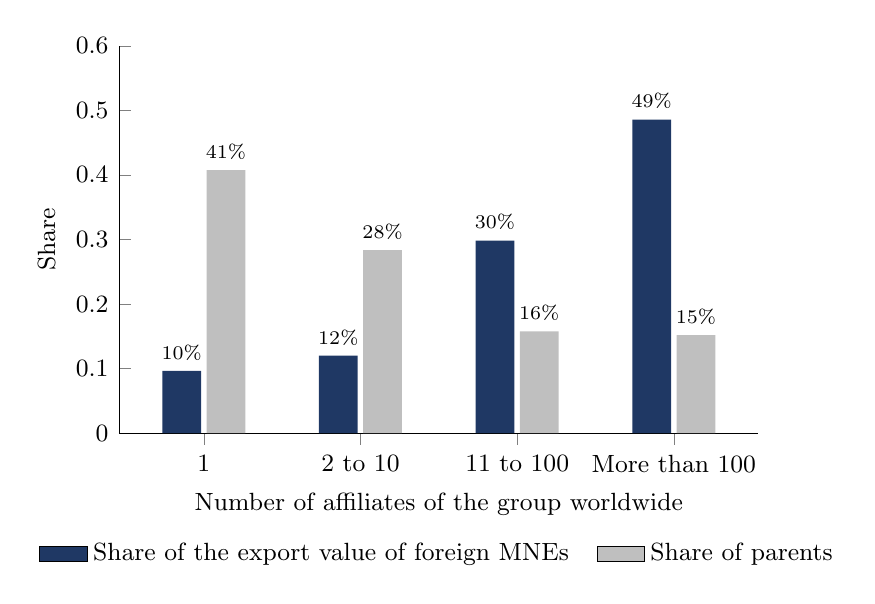
\begin{tikzpicture}
\begin{axis}[ybar, bar width=14pt, width=0.8\linewidth, height=6.5cm, ymin=0, ymax=0.6, ytick={0,0.1,0.2,0.3,0.4,0.5,0.6}, yticklabels={0,0.1,0.2,0.3,0.4,0.5,0.6},
  xtick={1,2,3,4}, xticklabels={{1},{2 to 10},{11 to 100},{More than 100}}, enlarge x limits=0.18,
  tick label style={font=\footnotesize}, xlabel={Number of affiliates of the group worldwide}, ylabel={Share}, label style={font=\footnotesize},
  axis x line*=bottom, axis y line*=left, nodes near coords={\pgfmathprintnumber[fixed,precision=0]{\pgfplotspointmeta}\%},
  point meta={100*y}, nodes near coords style={font=\scriptsize},
  area legend, legend image post style={draw=none}, legend cell align=left, legend style={at={(0.5,0)}, anchor=north, yshift=-1.25cm, draw=none, font=\footnotesize, legend columns=2, /tikz/every even column/.append style={column sep=8pt}}]
\addplot[fill={rgb,255:red,31;green,56;blue,100}, draw=none] coordinates {(1,0.0964) (2,0.1198) (3,0.2983) (4,0.4855)};
\addplot[fill={rgb,255:red,191;green,191;blue,191}, draw=none] coordinates {(1,0.4074) (2,0.2833) (3,0.1576) (4,0.1517)};
\legend{Share of the export value of foreign MNEs, Share of parents}
\end{axis}
\end{tikzpicture}}
{The figure shows the share of parents and the share of the exports of foreign MNEs by the number of affiliates of the
group worldwide in Orbis and Dun \& Bradstreet. Groups with this information account for 98 percent of the exports of
foreign MNEs.}{\srcnote}

\FloatBarrier
\section{Multinational Presence, Capital Intensity and Exports}\label{sec:regs}

In this section, we relate the presence of multinationals to exports over 2012 to 2018. We first estimate the
association between the number of multinationals and exports. We then ask whether it differs with capital intensity,
whether multinationals locate in capital intensive products, and what happens to local exports when the first
multinational enters.

\subsection{Exports are larger where more multinationals are present}\label{sec:base}

Exports are larger where more multinationals export the same product to the same destination. To assess this
association, we estimate
\begin{equation}\label{eq:presence}
\ln X_{odpy} = \beta \ln N_{odpy} + \delta + \varepsilon_{odpy},
\end{equation}
where $X_{odpy}$ is the value of product $p$ exported from origin $o$ to destination $d$ in year $y$, $N_{odpy}$ is the
number of MNEs that export it, and $\delta$ is a set of fixed effects. We estimate equation~(\ref{eq:presence}) on cells
with at least one MNE. We also replace $\ln N_{odpy}$ with an indicator for at least one MNE and estimate it on all cells.
The columns add fixed effects from origin, destination, product and year (column 1) to origin $\times$ destination
$\times$ product, origin $\times$ destination $\times$ year, origin $\times$ product $\times$ year and destination
$\times$ product $\times$ year (column 6).\footnote{Column 2 has origin $\times$ year, destination $\times$ year and
product fixed effects, column 3 origin $\times$ destination $\times$ product and year fixed effects, column 4 origin
$\times$ destination $\times$ product and origin $\times$ destination $\times$ year fixed effects, and column 5 adds
origin $\times$ product $\times$ year fixed effects. An accompanying workbook reports every specification, sample and
test.} In all specifications, we cluster standard errors by pair of origin and destination countries. Multinationals
choose the products and markets in which they operate, so these estimates are conditional correlations.

Table~\ref{tab:base} presents the estimates. The estimated coefficient on the number of multinationals is positive and
significant in all specifications. It falls from 2.19 to 0.83 once we follow the same origin, destination and product
over time (Panel A, columns 1 and 3). With origin $\times$ destination $\times$ year fixed effects, which control for
factors such as bilateral trade costs that vary over time, the estimate is 0.79. Specifically, a 10 percent increase in
the number of multinationals is associated with exports about 8 percent larger. This is true even under the most
demanding specification, which controls not only for these factors but also for shocks to each product in each origin
and in each destination. In this case, the estimate is 0.55. In Panel B, exports are 93 percent larger where at least
one multinational is present in column 4 and 78 percent larger in column 6. The exports of local firms are also larger
where more multinationals are present, with an elasticity of 0.37 in column 4 and 0.18 in column 6. This association
runs mainly through a larger number of local exporters (Appendix Tables~\ref{tab:a_local} and~\ref{tab:a_exporters}).

\vtab{tab:base}{Multinational presence and agricultural exports}{\begin{tabular}{l*{6}{c}}
\toprule
 & (1) & (2) & (3) & (4) & (5) & (6) \\
\midrule
\multicolumn{7}{l}{\textit{Panel A. Intensive margin: cells with at least one MNE}} \\
$\ln$(number of MNEs) & 2.194*** & 2.199*** & 0.827*** & 0.794*** & 0.702*** & 0.549*** \\
 & (0.029) & (0.029) & (0.022) & (0.022) & (0.022) & (0.031) \\
Observations (Panel A) & 101,309 & 101,195 & 90,311 & 88,525 & 82,787 & 32,982 \\
$R^2$ & 0.499 & 0.508 & 0.907 & 0.916 & 0.932 & 0.969 \\
\midrule
\multicolumn{7}{l}{\textit{Panel B. Extensive margin: all cells}} \\
At least one MNE & 1.824*** & 1.823*** & 0.661*** & 0.656*** & 0.616*** & 0.574*** \\
 & (0.065) & (0.064) & (0.027) & (0.026) & (0.025) & (0.036) \\
Observations (Panel B) & 198,148 & 198,063 & 177,873 & 176,192 & 169,531 & 90,414 \\
$R^2$ & 0.392 & 0.400 & 0.870 & 0.878 & 0.899 & 0.946 \\
\midrule
Origin FE & $\checkmark$ &  &  &  &  &  \\
Destination FE & $\checkmark$ &  &  &  &  &  \\
Product FE & $\checkmark$ & $\checkmark$ &  &  &  &  \\
Year FE & $\checkmark$ &  & $\checkmark$ &  &  &  \\
Origin $\times$ year FE &  & $\checkmark$ &  &  &  &  \\
Destination $\times$ year FE &  & $\checkmark$ &  &  &  &  \\
Origin $\times$ destination $\times$ product FE &  &  & $\checkmark$ & $\checkmark$ & $\checkmark$ & $\checkmark$ \\
Origin $\times$ destination $\times$ year FE &  &  &  & $\checkmark$ & $\checkmark$ & $\checkmark$ \\
Origin $\times$ product $\times$ year FE &  &  &  &  & $\checkmark$ & $\checkmark$ \\
Destination $\times$ product $\times$ year FE &  &  &  &  &  & $\checkmark$ \\
\bottomrule
\end{tabular}}
{The table reports estimated coefficients of equation~(\ref{eq:presence}) for 2012 to 2018. The dependent variable is
the natural logarithm of the exports of all firms. Panel A: cells with at least one MNE. Panel B: all cells. Standard
errors clustered by pair of origin and destination countries are reported in parentheses. \SIG}{\srcnote}

\FloatBarrier
\subsection{The association is stronger for farm products with high capital intensity}\label{sec:het}

We start by looking at the share of multinationals in the exports of products with different capital intensity
(Table~\ref{tab:quint} and Figure~\ref{fig:kl}). At the farm stage, multinationals ship a larger share of the exports
of products with more capital per worker. In 2018 they ship 36.7 percent of the exports of the farm products in the
lowest quintile, mostly fruit, and 64.7 percent of those in the fourth quintile, mostly grains and oilseeds. In
processing, the pattern does not hold. The share is 51.0 percent in the lowest quintile and 41.3 percent in the highest.

\vtab{tab:quint}{Multinational share of agricultural exports by capital intensity, 2018}{\begin{tabular}{lrrrrr}
\toprule
 & Products & Share of agricultural exports (\%) & MNE share (\%) & Foreign MNE share (\%) & Capital per worker (US\$ thousand) \\
\midrule
\textit{Farm stage} &  &  &  &  &  \\
Quintile 1 & 50 & 11.7 & 36.7 & 31.8 & 17 \\
Quintile 2 & 34 & 5.9 & 40.0 & 28.5 & 49 \\
Quintile 3 & 129 & 4.9 & 31.0 & 25.2 & 74 \\
Quintile 4 & 44 & 16.5 & 64.7 & 61.5 & 261 \\
Quintile 5 & 1 & 0.1 & 11.8 & 11.2 & 350 \\
\textit{Processing stage} &  &  &  &  &  \\
Quintile 1 & 169 & 18.2 & 51.0 & 39.0 & 75 \\
Quintile 2 & 180 & 9.7 & 49.3 & 41.2 & 125 \\
Quintile 3 & 76 & 8.4 & 48.0 & 37.2 & 172 \\
Quintile 4 & 50 & 20.8 & 41.9 & 33.4 & 250 \\
Quintile 5 & 23 & 2.8 & 41.3 & 37.4 & 277 \\
\bottomrule
\end{tabular}}
{The table reports the share of MNEs in the exports of each quintile of capital per worker within each stage. Quintiles
are weighted by exports of 2012 to 2018. Products linked to the same farm types or industries share one value, so
quintiles have unequal sizes. Capital per worker: average of the quintile weighted by exports.}{\textit{Source:} Authors' calculations based on customs data matched to Orbis (Bureau van Dijk) and Dun \& Bradstreet, USDA NASS, and NBER and CES.}

\vfig{fig:kl}{Multinational share of exports and capital per worker, by product, 2018}{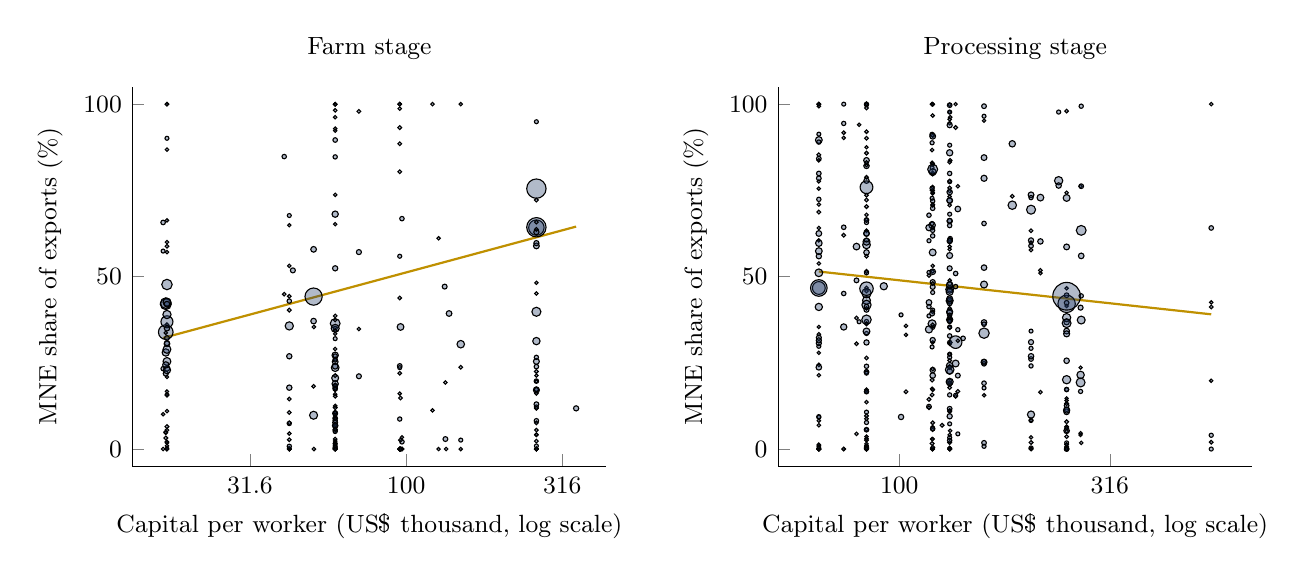
\begin{tikzpicture}
\begin{axis}[ width=7.6cm, height=6.4cm, xmode=log, log basis x=10, xmin=13.3, xmax=437.5, ymin=-5, ymax=105,
  xlabel={Capital per worker (US\$ thousand, log scale)}, ylabel={MNE share of exports (\%)}, title={Farm stage}, title style={font=\footnotesize},
  tick label style={font=\footnotesize}, label style={font=\footnotesize}, axis x line*=bottom, axis y line*=left, log ticks with fixed point,
  scatter/use mapped color={draw=none, fill={rgb,255:red,31;green,56;blue,100}, fill opacity=0.35}]
\addplot[scatter, only marks, mark=*, visualization depends on={\thisrow{s} \as \ps}, scatter/@pre marker code/.append style={/tikz/mark size=\ps}]
  table[x=x, y=y, meta=y, row sep=\\] {x y s \\ 95.37 8.7 0.78 \\ 95.37 80.4 0.66 \\ 95.37 0.0 0.60 \\ 95.37 24.1 0.84 \\ 149.56 2.6 0.73 \\ 149.56 30.4 1.36 \\ 149.56 0.0 0.61 \\ 149.56 100.0 0.60 \\ 121.45 100.0 0.64 \\ 121.45 11.2 0.62 \\ 127.00 61.1 0.62 \\ 127.00 0.0 0.60 \\ 96.94 2.1 0.81 \\ 96.94 0.0 0.67 \\ 96.94 0.0 0.61 \\ 96.94 0.0 0.60 \\ 95.93 0.0 0.60 \\ 95.93 0.0 0.63 \\ 95.37 100.0 0.62 \\ 95.93 14.8 0.66 \\ 95.93 2.6 0.70 \\ 95.93 0.0 0.61 \\ 95.93 0.0 0.63 \\ 95.93 0.0 0.62 \\ 50.66 0.0 0.65 \\ 50.66 35.4 0.65 \\ 42.25 7.4 0.76 \\ 42.25 4.5 0.64 \\ 42.25 64.9 0.60 \\ 42.25 2.7 0.66 \\ 42.25 53.1 0.63 \\ 42.25 40.3 0.71 \\ 42.25 14.5 0.65 \\ 42.25 35.7 1.49 \\ 42.25 0.0 0.62 \\ 95.37 98.7 0.62 \\ 95.37 16.1 0.62 \\ 95.37 0.0 0.66 \\ 95.37 23.6 0.72 \\ 95.37 0.0 0.61 \\ 95.37 100.0 0.61 \\ 95.37 100.0 0.62 \\ 95.37 55.9 0.73 \\ 95.37 93.2 0.70 \\ 42.25 67.7 0.72 \\ 42.25 0.0 0.60 \\ 42.25 0.0 0.60 \\ 42.25 42.9 0.81 \\ 42.25 7.6 0.71 \\ 95.37 43.8 0.65 \\ 95.37 0.0 0.63 \\ 42.25 0.0 0.60 \\ 42.25 0.0 0.60 \\ 42.25 0.0 0.61 \\ 95.37 0.0 0.63 \\ 95.37 88.5 0.68 \\ 95.37 0.0 0.60 \\ 42.25 0.3 0.60 \\ 95.37 0.0 0.61 \\ 95.93 0.0 0.60 \\ 42.25 10.6 0.69 \\ 95.37 22.0 0.66 \\ 133.55 2.9 0.88 \\ 133.55 19.3 0.64 \\ 96.94 66.8 0.81 \\ 96.94 3.4 0.60 \\ 95.93 35.4 1.22 \\ 95.93 0.0 0.63 \\ 42.25 0.2 0.62 \\ 149.56 23.7 0.68 \\ 132.82 47.1 0.89 \\ 16.67 23.3 0.78 \\ 16.67 0.0 0.63 \\ 16.67 65.7 0.83 \\ 16.67 57.4 0.73 \\ 16.67 10.1 0.61 \\ 42.25 17.8 0.97 \\ 59.26 23.6 1.39 \\ 59.26 20.6 1.25 \\ 59.26 0.0 0.63 \\ 59.26 18.9 1.14 \\ 59.26 8.9 0.83 \\ 59.26 36.4 1.77 \\ 59.26 0.3 0.80 \\ 70.58 21.1 0.90 \\ 59.26 2.3 0.64 \\ 59.26 17.8 0.69 \\ 59.26 5.5 0.80 \\ 59.26 25.3 1.04 \\ 59.26 27.2 1.14 \\ 59.26 18.5 0.66 \\ 59.26 37.4 0.62 \\ 59.26 2.9 0.64 \\ 59.26 9.2 0.64 \\ 59.26 17.8 0.63 \\ 59.26 18.6 0.65 \\ 59.26 100.0 0.61 \\ 59.26 92.9 0.61 \\ 59.26 35.0 0.73 \\ 59.26 10.1 0.63 \\ 59.26 1.6 0.73 \\ 261.16 8.2 0.81 \\ 261.16 11.8 0.67 \\ 261.16 4.2 0.62 \\ 59.26 35.0 1.45 \\ 59.26 34.3 0.68 \\ 59.26 6.6 0.64 \\ 59.26 12.5 0.65 \\ 59.26 38.6 0.65 \\ 59.26 18.3 0.81 \\ 59.26 17.1 0.62 \\ 59.26 92.3 0.61 \\ 59.26 7.0 0.71 \\ 59.26 7.7 0.89 \\ 261.16 19.7 0.81 \\ 261.16 25.4 1.07 \\ 261.16 23.9 0.82 \\ 261.16 19.6 0.65 \\ 261.16 31.3 1.33 \\ 261.16 48.2 0.60 \\ 261.16 17.4 0.77 \\ 261.16 16.1 0.65 \\ 261.16 2.3 0.68 \\ 261.16 0.0 0.60 \\ 261.16 7.6 0.69 \\ 59.26 6.8 1.00 \\ 59.26 5.1 0.75 \\ 59.26 8.3 0.79 \\ 59.26 12.0 0.71 \\ 59.26 32.0 0.72 \\ 59.26 5.7 0.69 \\ 17.15 0.0 0.61 \\ 17.15 15.9 0.65 \\ 17.15 0.9 0.62 \\ 17.15 66.3 0.60 \\ 17.15 57.1 0.63 \\ 17.15 100.0 0.65 \\ 17.15 30.5 1.03 \\ 17.15 58.8 0.66 \\ 17.15 1.8 0.65 \\ 17.15 36.1 0.63 \\ 17.15 6.5 0.70 \\ 17.00 21.9 0.93 \\ 17.00 33.9 2.64 \\ 17.00 4.7 0.64 \\ 17.00 3.2 0.71 \\ 17.00 42.0 1.98 \\ 17.00 42.3 1.94 \\ 17.00 28.0 1.33 \\ 17.15 23.4 1.03 \\ 17.15 22.9 1.31 \\ 17.15 32.2 0.87 \\ 17.15 90.1 0.72 \\ 17.15 15.6 0.67 \\ 17.15 28.9 1.42 \\ 17.15 0.3 0.61 \\ 17.15 36.9 2.17 \\ 59.26 17.5 0.83 \\ 59.26 52.4 0.95 \\ 17.00 4.9 0.69 \\ 17.15 39.0 1.49 \\ 17.15 25.4 1.42 \\ 17.15 11.0 0.63 \\ 17.15 60.0 0.64 \\ 17.15 20.9 0.61 \\ 17.15 42.6 1.43 \\ 17.15 30.7 0.93 \\ 17.15 35.0 0.97 \\ 17.15 5.5 0.66 \\ 17.15 2.1 0.63 \\ 17.15 47.7 1.89 \\ 17.15 42.0 1.03 \\ 17.00 33.7 0.61 \\ 17.15 86.8 0.63 \\ 17.00 24.4 1.14 \\ 50.54 44.2 3.11 \\ 50.54 18.2 0.66 \\ 50.54 37.1 1.01 \\ 50.54 57.9 1.03 \\ 59.26 0.9 0.67 \\ 59.26 98.2 0.64 \\ 59.26 29.0 0.63 \\ 59.26 15.9 0.63 \\ 59.26 0.0 0.61 \\ 59.26 1.6 0.62 \\ 59.26 10.8 0.62 \\ 59.26 0.0 0.62 \\ 59.26 1.2 0.64 \\ 59.26 17.5 0.70 \\ 59.26 0.0 0.62 \\ 59.26 65.2 0.60 \\ 59.26 10.3 0.89 \\ 59.26 33.4 0.60 \\ 59.26 21.3 0.69 \\ 59.26 8.8 0.63 \\ 59.26 26.1 0.72 \\ 261.16 0.9 0.72 \\ 261.16 64.2 2.80 \\ 261.16 45.1 0.61 \\ 261.16 39.8 1.64 \\ 261.16 0.0 0.63 \\ 261.16 72.2 0.69 \\ 261.16 58.9 1.05 \\ 261.16 64.3 3.50 \\ 350.04 11.8 0.94 \\ 261.16 59.7 0.93 \\ 261.16 21.3 0.61 \\ 261.16 0.0 0.60 \\ 261.16 4.1 0.62 \\ 261.16 12.2 0.74 \\ 261.16 5.5 0.63 \\ 261.16 17.1 1.09 \\ 261.16 75.5 3.50 \\ 261.16 0.0 0.61 \\ 261.16 0.0 0.61 \\ 17.15 16.7 0.60 \\ 261.16 22.5 0.70 \\ 261.16 17.2 0.78 \\ 261.16 26.6 0.77 \\ 261.16 62.9 0.95 \\ 17.15 0.0 0.70 \\ 261.16 63.7 0.67 \\ 261.16 0.0 0.60 \\ 261.16 13.0 0.86 \\ 261.16 94.9 0.72 \\ 261.16 0.0 0.60 \\ 261.16 65.8 0.67 \\ 261.16 0.0 0.60 \\ 137.18 39.3 1.03 \\ 59.26 100.0 0.60 \\ 59.26 73.7 0.62 \\ 59.26 10.6 0.71 \\ 59.26 15.3 0.66 \\ 59.26 0.0 0.60 \\ 59.26 27.0 0.76 \\ 59.26 25.8 0.76 \\ 59.26 84.7 0.78 \\ 59.26 68.1 1.14 \\ 40.70 84.8 0.80 \\ 59.26 96.2 0.62 \\ 59.26 99.9 0.61 \\ 59.26 0.0 0.64 \\ 59.26 24.0 1.02 \\ 42.25 44.3 0.65 \\ 42.25 26.9 0.96 \\ 59.26 0.7 0.61 \\ 17.15 100.0 0.60 \\ 134.26 0.0 0.63 \\ 40.70 44.9 0.65 \\ 261.16 0.0 0.60 \\ 59.26 89.6 0.83 \\ 59.26 0.0 0.62 \\ 42.25 0.8 0.78 \\ 70.58 34.8 0.63 \\ 70.58 97.9 0.70 \\ 70.58 57.1 0.92 \\ 50.54 9.8 1.45 \\ 43.38 51.8 0.91 \\};
\addplot[thick, color={rgb,255:red,191;green,144;blue,0}, no marks] coordinates {(16.67,32.21) (19.57,33.91) (22.97,35.61) (26.96,37.31) (31.65,39.00) (37.15,40.70) (43.60,42.40) (51.18,44.10) (60.07,45.80) (70.51,47.50) (82.77,49.20) (97.15,50.90) (114.03,52.60) (133.85,54.30) (157.11,56.00) (184.41,57.70) (216.45,59.40) (254.07,61.10) (298.22,62.80) (350.04,64.50)};
\end{axis}
\begin{axis}[xshift=8.2cm, width=7.6cm, height=6.4cm, xmode=log, log basis x=10, xmin=51.6, xmax=688.1, ymin=-5, ymax=105,
  xlabel={Capital per worker (US\$ thousand, log scale)}, ylabel={MNE share of exports (\%)}, title={Processing stage}, title style={font=\footnotesize},
  tick label style={font=\footnotesize}, label style={font=\footnotesize}, axis x line*=bottom, axis y line*=left, log ticks with fixed point,
  scatter/use mapped color={draw=none, fill={rgb,255:red,31;green,56;blue,100}, fill opacity=0.35}]
\addplot[scatter, only marks, mark=*, visualization depends on={\thisrow{s} \as \ps}, scatter/@pre marker code/.append style={/tikz/mark size=\ps}]
  table[x=x, y=y, meta=y, row sep=\\] {x y s \\ 64.45 100.0 0.60 \\ 64.45 91.3 0.72 \\ 64.45 46.7 2.32 \\ 64.45 60.5 0.62 \\ 64.45 59.7 1.19 \\ 64.45 46.7 3.00 \\ 64.45 0.0 0.60 \\ 64.45 27.9 0.60 \\ 64.45 8.2 0.60 \\ 64.45 0.0 0.71 \\ 64.45 79.9 0.84 \\ 64.45 89.6 1.23 \\ 64.45 77.6 0.60 \\ 64.45 0.0 0.61 \\ 64.45 0.0 0.60 \\ 64.45 29.8 0.74 \\ 64.45 24.4 0.68 \\ 64.45 55.9 0.96 \\ 64.45 72.4 0.79 \\ 64.45 0.1 0.62 \\ 64.45 62.5 1.04 \\ 64.45 9.2 0.72 \\ 64.45 32.3 0.92 \\ 64.45 30.7 0.93 \\ 64.45 41.2 1.32 \\ 64.45 75.5 0.62 \\ 64.45 64.1 0.63 \\ 64.45 84.2 0.85 \\ 64.45 70.9 0.64 \\ 64.45 85.3 0.71 \\ 64.45 0.9 0.68 \\ 64.45 23.7 1.01 \\ 64.45 1.3 0.60 \\ 64.45 51.1 1.40 \\ 64.45 100.0 0.63 \\ 64.45 6.9 0.64 \\ 64.45 0.0 0.60 \\ 64.45 78.5 0.86 \\ 64.45 0.0 0.60 \\ 64.45 35.4 0.60 \\ 64.45 0.0 0.60 \\ 64.45 0.0 0.60 \\ 64.45 9.4 0.74 \\ 64.45 100.0 0.61 \\ 64.45 33.3 0.63 \\ 64.45 89.0 0.79 \\ 64.45 0.0 0.61 \\ 64.45 0.5 0.62 \\ 64.45 99.4 0.63 \\ 64.45 83.7 0.63 \\ 64.45 100.0 0.65 \\ 64.45 68.7 0.69 \\ 83.63 0.0 0.60 \\ 83.63 43.1 1.43 \\ 83.63 59.2 1.41 \\ 83.63 82.1 0.98 \\ 83.63 3.6 0.62 \\ 83.63 82.3 0.62 \\ 83.63 66.6 0.63 \\ 83.63 100.0 0.60 \\ 83.63 0.7 0.61 \\ 83.63 0.0 0.61 \\ 83.63 51.5 0.71 \\ 83.63 8.8 0.67 \\ 83.63 90.1 0.68 \\ 83.63 46.7 0.69 \\ 83.63 5.7 0.61 \\ 83.63 0.5 0.62 \\ 83.63 33.5 0.74 \\ 83.63 34.1 1.23 \\ 83.63 63.3 0.65 \\ 83.63 0.0 0.61 \\ 83.63 62.5 1.02 \\ 83.63 87.5 0.62 \\ 83.63 73.6 0.66 \\ 83.63 37.0 0.75 \\ 83.63 78.8 0.64 \\ 83.63 83.7 1.02 \\ 83.63 30.9 0.96 \\ 83.63 24.0 0.79 \\ 83.63 0.4 0.74 \\ 83.63 57.0 1.00 \\ 83.63 41.8 1.68 \\ 83.63 65.7 0.77 \\ 83.63 92.0 0.64 \\ 83.63 1.0 0.64 \\ 83.63 0.0 0.68 \\ 83.63 100.0 0.66 \\ 83.63 22.3 0.80 \\ 83.63 100.0 0.63 \\ 83.63 55.9 0.68 \\ 83.63 0.0 0.61 \\ 83.63 16.7 0.70 \\ 83.63 98.9 0.67 \\ 83.63 99.8 0.73 \\ 83.63 100.0 0.75 \\ 83.63 37.5 1.71 \\ 83.63 77.8 0.96 \\ 83.63 13.6 0.64 \\ 83.63 7.7 0.75 \\ 83.63 0.0 0.60 \\ 83.63 45.8 0.68 \\ 83.63 17.2 0.67 \\ 83.63 9.6 0.71 \\ 83.63 36.3 0.69 \\ 83.63 85.8 0.68 \\ 83.63 60.1 1.26 \\ 83.63 100.0 0.60 \\ 83.63 51.1 0.76 \\ 83.63 0.0 0.60 \\ 83.63 0.2 0.75 \\ 83.63 22.4 0.82 \\ 83.63 2.6 0.70 \\ 83.63 22.0 0.72 \\ 83.63 0.0 0.61 \\ 83.63 0.8 0.67 \\ 83.63 0.0 0.60 \\ 83.63 0.0 0.63 \\ 83.63 10.7 0.74 \\ 83.63 1.5 0.61 \\ 83.63 16.6 0.78 \\ 83.63 0.0 0.60 \\ 83.63 0.0 0.60 \\ 83.63 0.0 0.68 \\ 83.63 0.3 0.66 \\ 83.63 0.0 0.62 \\ 83.63 0.6 0.70 \\ 83.63 40.4 0.92 \\ 83.63 0.0 0.61 \\ 83.63 75.9 2.31 \\ 83.63 40.8 0.64 \\ 83.63 60.6 0.74 \\ 83.63 41.3 0.85 \\ 83.63 100.0 0.61 \\ 83.63 3.0 0.62 \\ 83.63 62.5 1.00 \\ 83.63 5.6 0.82 \\ 83.63 72.2 0.69 \\ 83.63 99.9 0.62 \\ 83.63 67.9 0.65 \\ 83.63 0.2 0.65 \\ 83.63 83.1 0.68 \\ 83.63 45.2 1.69 \\ 83.63 100.0 0.62 \\ 83.63 66.4 0.82 \\ 158.99 0.8 0.75 \\ 158.99 36.7 1.01 \\ 158.99 33.6 1.88 \\ 158.99 15.6 0.63 \\ 158.99 84.5 1.05 \\ 158.99 99.4 0.86 \\ 158.99 36.2 0.82 \\ 158.99 17.7 0.72 \\ 158.99 52.6 1.01 \\ 158.99 19.1 0.82 \\ 158.99 25.2 1.08 \\ 158.99 95.2 0.60 \\ 158.99 65.4 0.82 \\ 158.99 78.5 1.11 \\ 158.99 24.7 0.81 \\ 158.99 1.8 0.85 \\ 158.99 96.5 0.72 \\ 158.99 47.7 1.26 \\ 120.08 7.6 0.68 \\ 120.08 96.7 0.64 \\ 120.08 35.3 0.74 \\ 120.08 30.9 0.64 \\ 64.45 57.4 1.22 \\ 83.63 70.3 0.70 \\ 131.76 46.7 0.66 \\ 131.76 30.5 0.64 \\ 131.76 60.0 0.69 \\ 131.76 37.7 0.66 \\ 131.76 43.0 0.61 \\ 131.76 27.5 0.73 \\ 131.76 39.5 1.02 \\ 131.76 77.5 0.72 \\ 131.76 18.8 0.75 \\ 131.76 10.8 0.63 \\ 131.76 99.8 0.62 \\ 131.76 37.1 0.64 \\ 131.76 23.6 0.68 \\ 131.76 60.9 0.66 \\ 131.76 74.8 0.65 \\ 131.76 25.7 0.69 \\ 131.76 30.9 0.76 \\ 131.76 19.7 0.75 \\ 131.76 9.5 0.95 \\ 131.76 0.0 0.63 \\ 131.76 32.8 0.81 \\ 131.76 99.7 0.84 \\ 131.76 22.5 1.02 \\ 131.76 48.9 0.62 \\ 131.76 0.0 0.60 \\ 131.76 0.3 0.65 \\ 131.76 37.5 1.12 \\ 131.76 37.4 0.91 \\ 131.76 46.3 0.93 \\ 131.76 46.3 1.41 \\ 131.76 19.3 0.66 \\ 131.76 3.3 0.73 \\ 131.76 4.1 0.62 \\ 131.76 39.8 1.10 \\ 131.76 79.9 0.80 \\ 131.76 26.6 0.75 \\ 131.76 40.8 0.63 \\ 131.76 7.3 0.73 \\ 120.08 40.3 0.72 \\ 120.08 22.9 0.96 \\ 120.08 70.6 0.62 \\ 120.08 53.1 0.63 \\ 120.08 23.2 0.67 \\ 120.08 39.8 0.68 \\ 120.08 80.1 0.64 \\ 120.08 21.3 1.01 \\ 120.08 0.0 0.60 \\ 120.08 82.7 0.63 \\ 120.08 100.0 0.60 \\ 120.08 76.0 0.61 \\ 120.08 100.0 0.60 \\ 120.08 0.0 0.61 \\ 120.08 99.9 0.60 \\ 120.08 75.0 0.62 \\ 120.08 6.4 0.62 \\ 120.08 51.5 0.61 \\ 205.56 73.7 1.05 \\ 205.56 69.4 1.63 \\ 205.56 60.5 0.94 \\ 205.56 10.0 1.30 \\ 205.56 31.0 0.93 \\ 205.56 59.8 0.68 \\ 205.56 0.3 0.76 \\ 205.56 8.3 0.75 \\ 205.56 0.1 0.61 \\ 205.56 0.0 0.60 \\ 205.56 58.9 0.84 \\ 205.56 8.3 0.63 \\ 205.56 72.9 0.77 \\ 205.56 29.2 0.74 \\ 205.56 63.3 0.68 \\ 205.56 0.0 0.61 \\ 131.76 0.3 0.62 \\ 131.76 24.0 0.63 \\ 205.56 57.7 0.66 \\ 205.56 24.1 0.77 \\ 205.56 34.2 0.72 \\ 239.05 77.8 1.50 \\ 239.05 97.7 0.75 \\ 550.45 0.0 0.73 \\ 550.45 64.1 0.83 \\ 550.45 19.8 0.62 \\ 550.45 4.0 0.76 \\ 550.45 42.5 0.62 \\ 550.45 100.0 0.65 \\ 550.45 2.0 0.67 \\ 131.76 24.2 1.16 \\ 249.69 6.5 0.70 \\ 249.69 41.5 0.63 \\ 185.55 73.3 0.66 \\ 120.08 2.9 0.60 \\ 120.08 0.0 0.62 \\ 120.08 0.0 0.61 \\ 120.08 61.8 0.80 \\ 120.08 74.1 0.62 \\ 120.08 74.4 0.62 \\ 120.08 47.0 0.90 \\ 249.69 0.0 0.61 \\ 64.45 21.4 0.63 \\ 249.69 36.8 0.98 \\ 64.45 53.8 0.63 \\ 249.69 0.0 0.62 \\ 249.69 0.6 0.62 \\ 249.69 38.1 1.50 \\ 80.33 36.9 0.73 \\ 80.33 94.0 0.61 \\ 249.69 42.1 3.15 \\ 249.69 58.6 1.06 \\ 249.69 5.3 1.01 \\ 249.69 14.1 0.62 \\ 249.69 34.2 1.04 \\ 249.69 1.8 0.72 \\ 249.69 0.1 0.60 \\ 249.69 36.5 1.60 \\ 249.69 10.8 1.03 \\ 249.69 20.1 1.50 \\ 249.69 33.4 1.10 \\ 249.69 0.6 0.69 \\ 249.69 46.6 0.61 \\ 249.69 3.6 0.67 \\ 249.69 25.6 1.00 \\ 249.69 12.6 0.85 \\ 249.69 17.2 0.74 \\ 249.69 1.3 0.66 \\ 249.69 0.0 0.60 \\ 249.69 0.0 0.61 \\ 249.69 0.0 0.76 \\ 249.69 11.5 0.79 \\ 249.69 5.2 0.66 \\ 249.69 14.7 0.61 \\ 249.69 74.3 0.61 \\ 249.69 44.6 0.85 \\ 249.69 0.0 0.83 \\ 249.69 17.3 0.76 \\ 249.69 42.4 0.84 \\ 249.69 72.8 1.24 \\ 249.69 1.3 0.63 \\ 249.69 6.1 0.69 \\ 249.69 0.0 0.62 \\ 73.85 64.3 0.82 \\ 120.08 90.8 0.62 \\ 73.85 0.0 0.60 \\ 73.85 94.4 0.78 \\ 73.85 45.1 0.81 \\ 73.85 0.0 0.67 \\ 73.85 90.2 0.62 \\ 73.85 100.0 0.72 \\ 73.85 62.0 0.70 \\ 73.85 35.4 1.14 \\ 73.85 91.7 0.64 \\ 120.08 79.7 0.65 \\ 119.69 81.5 0.74 \\ 119.69 2.9 0.62 \\ 119.69 20.0 0.71 \\ 119.69 64.9 1.18 \\ 119.69 75.0 0.67 \\ 119.69 39.3 0.90 \\ 119.69 91.2 0.80 \\ 119.69 75.6 0.77 \\ 83.63 26.4 0.69 \\ 119.69 29.6 0.73 \\ 119.69 65.4 0.73 \\ 119.69 15.7 0.70 \\ 119.69 1.6 0.71 \\ 119.69 36.3 1.46 \\ 119.69 86.7 0.65 \\ 119.69 17.5 0.62 \\ 119.69 83.0 0.66 \\ 119.69 72.7 0.72 \\ 119.69 88.8 0.75 \\ 119.69 100.0 0.61 \\ 119.69 100.0 0.62 \\ 119.69 0.0 0.62 \\ 269.52 76.2 0.61 \\ 269.52 16.7 0.77 \\ 269.52 19.3 1.61 \\ 269.52 4.1 0.61 \\ 269.52 21.5 1.34 \\ 132.12 96.2 0.65 \\ 132.12 5.3 0.61 \\ 269.52 23.6 0.60 \\ 132.12 61.0 0.81 \\ 132.12 83.7 0.65 \\ 132.12 0.0 0.62 \\ 132.12 30.9 0.68 \\ 132.12 60.5 0.81 \\ 269.52 41.0 0.92 \\ 269.52 4.6 0.61 \\ 117.67 60.4 0.75 \\ 117.67 34.7 1.31 \\ 117.67 38.6 0.74 \\ 117.67 50.3 0.66 \\ 117.67 42.5 1.02 \\ 117.67 67.8 0.80 \\ 117.67 14.4 0.69 \\ 117.67 41.3 0.80 \\ 117.67 51.2 0.74 \\ 117.67 12.3 0.85 \\ 117.67 64.2 1.14 \\ 120.08 90.7 1.06 \\ 205.56 26.1 0.84 \\ 120.08 51.4 1.02 \\ 101.01 38.9 0.74 \\ 101.01 9.3 0.97 \\ 103.75 16.6 0.68 \\ 103.75 35.7 0.65 \\ 103.75 33.1 0.61 \\ 550.45 41.2 0.66 \\ 205.56 26.9 0.99 \\ 205.56 1.9 0.70 \\ 205.56 3.4 0.62 \\ 141.78 32.1 0.83 \\ 79.19 4.4 0.62 \\ 79.19 30.5 0.66 \\ 79.19 58.7 1.21 \\ 79.19 48.9 0.87 \\ 79.19 38.0 0.68 \\ 91.92 47.2 1.31 \\ 131.76 73.2 0.62 \\ 131.76 72.0 0.99 \\ 131.76 11.2 0.65 \\ 131.76 66.1 0.97 \\ 131.76 70.7 0.63 \\ 131.76 57.9 0.61 \\ 131.76 85.9 1.14 \\ 126.41 6.9 0.68 \\ 120.08 5.6 0.63 \\ 131.76 64.8 0.80 \\ 131.76 68.1 0.73 \\ 131.76 1.9 0.70 \\ 131.76 2.5 0.81 \\ 131.76 72.1 1.03 \\ 131.76 43.0 1.02 \\ 131.76 17.8 0.67 \\ 131.76 0.0 0.60 \\ 131.76 43.0 1.28 \\ 117.67 12.0 0.68 \\ 120.08 69.8 0.82 \\ 131.76 58.7 0.63 \\ 131.76 56.1 1.09 \\ 131.76 23.0 1.56 \\ 131.76 11.7 0.84 \\ 131.76 75.7 0.67 \\ 131.76 42.2 0.83 \\ 131.76 94.5 0.65 \\ 131.76 0.0 0.61 \\ 131.76 35.2 0.70 \\ 131.76 60.3 0.94 \\ 131.76 77.7 0.67 \\ 131.76 38.8 0.79 \\ 131.76 88.1 0.73 \\ 131.76 37.0 0.80 \\ 131.76 45.6 1.28 \\ 131.76 48.0 0.79 \\ 131.76 11.0 0.71 \\ 131.76 93.9 0.94 \\ 131.76 97.7 0.61 \\ 131.76 35.4 0.73 \\ 131.76 38.3 0.62 \\ 131.76 19.5 1.28 \\ 131.76 74.5 0.98 \\ 131.76 66.2 0.85 \\ 131.76 95.6 0.63 \\ 131.76 27.5 0.65 \\ 131.76 47.6 1.17 \\ 131.76 97.7 0.73 \\ 131.76 52.4 0.91 \\ 131.76 83.2 0.71 \\ 131.76 43.6 1.06 \\ 131.76 15.7 0.77 \\ 120.08 80.3 1.25 \\ 120.08 45.4 0.74 \\ 120.08 71.9 0.78 \\ 120.08 82.6 0.68 \\ 120.08 48.4 0.92 \\ 120.08 48.0 0.67 \\ 120.08 64.1 0.67 \\ 120.08 36.0 0.67 \\ 120.08 31.6 0.95 \\ 120.08 70.9 0.68 \\ 120.08 57.0 1.24 \\ 120.08 63.4 0.78 \\ 120.08 0.5 0.71 \\ 158.99 25.3 0.85 \\ 120.08 5.9 0.81 \\ 120.08 81.1 1.80 \\ 216.39 16.5 0.64 \\ 216.39 51.8 0.68 \\ 216.39 60.2 0.99 \\ 216.39 51.0 0.61 \\ 216.39 72.9 1.22 \\ 239.05 76.4 0.99 \\ 136.13 50.9 0.82 \\ 136.13 31.0 2.28 \\ 136.13 47.1 0.79 \\ 136.13 24.8 1.24 \\ 136.13 93.2 0.71 \\ 136.13 15.3 0.67 \\ 136.13 100.0 0.60 \\ 136.13 15.6 0.73 \\ 137.78 34.6 0.77 \\ 137.78 16.7 0.69 \\ 137.78 69.6 1.02 \\ 137.78 31.4 0.63 \\ 137.78 76.2 0.64 \\ 137.78 4.4 0.73 \\ 137.78 21.3 0.88 \\ 120.08 17.2 0.67 \\ 64.45 31.5 0.94 \\ 83.63 46.5 2.43 \\ 249.69 44.3 5.00 \\ 249.69 7.9 0.69 \\ 249.69 98.0 0.66 \\ 249.69 0.0 0.63 \\ 249.69 11.3 1.12 \\ 249.69 0.0 0.61 \\ 249.69 0.0 0.62 \\ 249.69 0.0 0.62 \\ 249.69 0.0 0.66 \\ 249.69 13.2 0.69 \\ 185.55 88.5 1.16 \\ 185.55 70.7 1.53 \\ 270.43 37.4 1.43 \\ 270.43 63.4 1.78 \\ 270.43 56.0 1.02 \\ 270.43 1.8 0.63 \\ 270.43 44.4 0.79 \\ 270.43 76.2 0.85 \\ 270.43 99.4 0.78 \\};
\addplot[thick, color={rgb,255:red,191;green,144;blue,0}, no marks] coordinates {(64.45,51.47) (72.15,50.81) (80.77,50.16) (90.43,49.51) (101.23,48.86) (113.33,48.20) (126.88,47.55) (142.04,46.90) (159.01,46.24) (178.01,45.59) (199.29,44.94) (223.10,44.29) (249.77,43.63) (279.61,42.98) (313.03,42.33) (350.44,41.67) (392.32,41.02) (439.20,40.37) (491.69,39.72) (550.45,39.06)};
\end{axis}
\end{tikzpicture}}
{The figure shows the MNE share of the exports of each product against its capital per worker. Each marker is an HS6
product, with size proportional to its exports. The line is a fit weighted by exports.}{\textit{Source:} Authors' calculations based on customs data matched to Orbis (Bureau van Dijk) and Dun \& Bradstreet, USDA NASS, and NBER and CES.}

The association between multinational presence and exports follows the same pattern. Table~\ref{tab:het} reports
estimates of equation~(\ref{eq:presence}) in which we interact $\ln N_{odpy}$ with indicators for groups of products.
With the stages pooled, products with high capital intensity show a larger elasticity, 0.83 against 0.76 in column 2.
However, the difference is small, and it is not significant in the strictest specification (Panel A). With the median
as the threshold, the difference is larger and significant in every column, 1.00 against 0.74 in column 2 and 0.78
against 0.51 in column 4 (Panel B). Panel C shows that the difference comes from farm products. The elasticity is 1.11
for farm products with high capital intensity and 0.66 for the other farm products in column 2, and 1.10 against 0.50 in
column 4. Among processed products, the order depends on the threshold, and the difference is not significant in the
strictest specification (Panel C and Appendix Table~\ref{tab:a_hetmed}).

\vtab{tab:het}{Multinational presence and agricultural exports, by capital intensity}{\begin{tabular}{l*{4}{c}}
\toprule
 & (1) & (2) & (3) & (4) \\
\midrule
\multicolumn{5}{l}{\textit{Panel A. Stages pooled, threshold: aggregate ratio of the stage}} \\
$\ln$(number of MNEs) $\times$ high capital intensity & 0.853*** & 0.829*** & 0.743*** & 0.570*** \\
 & (0.029) & (0.029) & (0.031) & (0.046) \\
$\ln$(number of MNEs) $\times$ low capital intensity & 0.799*** & 0.756*** & 0.653*** & 0.531*** \\
 & (0.030) & (0.029) & (0.025) & (0.038) \\
$\ln$(number of MNEs) $\times$ not classified & 0.861*** & 0.873*** & 0.949*** & 0.001 \\
 & (0.140) & (0.143) & (0.154) & (0.512) \\
$p$ value: high = low & 0.140 & 0.051 & 0.011 & 0.502 \\
Observations (Panel A) & 90,311 & 88,525 & 82,787 & 32,982 \\
$R^2$ & 0.907 & 0.916 & 0.933 & 0.969 \\
\midrule
\multicolumn{5}{l}{\textit{Panel B. Stages pooled, threshold: export weighted median of the stage}} \\
$\ln$(number of MNEs) $\times$ high capital intensity & 1.014*** & 0.995*** & 0.921*** & 0.783*** \\
 & (0.042) & (0.044) & (0.050) & (0.080) \\
$\ln$(number of MNEs) $\times$ low capital intensity & 0.775*** & 0.738*** & 0.640*** & 0.512*** \\
 & (0.023) & (0.022) & (0.020) & (0.034) \\
$\ln$(number of MNEs) $\times$ not classified & 0.861*** & 0.874*** & 0.949*** & 0.002 \\
 & (0.140) & (0.143) & (0.153) & (0.513) \\
$p$ value: high = low & 0.000 & 0.000 & 0.000 & 0.002 \\
Observations (Panel B) & 90,311 & 88,525 & 82,787 & 32,982 \\
$R^2$ & 0.907 & 0.916 & 0.933 & 0.969 \\
\midrule
\multicolumn{5}{l}{\textit{Panel C. By stage, threshold: aggregate ratio of the stage}} \\
$\ln$(number of MNEs) $\times$ farm stage, high & 1.135*** & 1.111*** & 1.045*** & 1.095*** \\
 & (0.058) & (0.059) & (0.068) & (0.129) \\
$\ln$(number of MNEs) $\times$ farm stage, low & 0.710*** & 0.661*** & 0.590*** & 0.499*** \\
 & (0.036) & (0.033) & (0.031) & (0.052) \\
$\ln$(number of MNEs) $\times$ processing stage, high & 0.781*** & 0.758*** & 0.668*** & 0.511*** \\
 & (0.029) & (0.028) & (0.029) & (0.051) \\
$\ln$(number of MNEs) $\times$ processing stage, low & 0.917*** & 0.877*** & 0.735*** & 0.565*** \\
 & (0.039) & (0.040) & (0.037) & (0.057) \\
$\ln$(number of MNEs) $\times$ not classified & 0.861*** & 0.872*** & 0.950*** & -0.028 \\
 & (0.140) & (0.144) & (0.154) & (0.509) \\
$p$ value: farm stage, high = low & 0.000 & 0.000 & 0.000 & 0.000 \\
$p$ value: processing stage, high = low & 0.003 & 0.013 & 0.144 & 0.443 \\
Observations (Panel C) & 90,311 & 88,525 & 82,787 & 32,982 \\
$R^2$ & 0.907 & 0.916 & 0.933 & 0.969 \\
\midrule
Year FE & $\checkmark$ &  &  &  \\
Origin $\times$ destination $\times$ product FE & $\checkmark$ & $\checkmark$ & $\checkmark$ & $\checkmark$ \\
Origin $\times$ destination $\times$ year FE &  & $\checkmark$ & $\checkmark$ & $\checkmark$ \\
Origin $\times$ product $\times$ year FE &  &  & $\checkmark$ & $\checkmark$ \\
Destination $\times$ product $\times$ year FE &  &  &  & $\checkmark$ \\
\bottomrule
\end{tabular}}
{The table reports estimated coefficients of equation~(\ref{eq:presence}) with the natural logarithm of the number of
MNEs interacted with an indicator for each group of products. Cells with at least one MNE. Columns 1 to 4 have the fixed
effects of columns 3 to 6 of Table~\ref{tab:base}. Standard errors clustered by pair of origin and destination countries
are reported in parentheses. \SIG}{\textit{Source:} Authors' calculations based on customs data matched to Orbis (Bureau van Dijk) and Dun \& Bradstreet, USDA NASS, and NBER and CES.}

At the farm stage, capital intensity and the type of production go together, as most farm products with high capital
intensity are field crops. In Table~\ref{tab:farm}, we therefore add the interactions with the type of production. The
difference between farm products with high and low capital intensity remains, 1.15 against 0.81 in column 2. It is
significant in columns 1 to 3 but not in the strictest specification (Panel A). The continuous measure of capital per
worker shows no slope once we control for the type of production (Panel B). With the stages pooled, the elasticity rises
by 0.09 for each log point of capital per worker in column 2, and the slope is not significant in the strictest
specification (Appendix Table~\ref{tab:a_cont}). Thus, the stronger association is a feature of a group of farm
products, mainly grains and oilseeds, and not a gradient along capital per worker.

\vtab{tab:farm}{Multinational presence and the exports of farm products: capital intensity and type of production}{\begin{tabular}{l*{4}{c}}
\toprule
 & (1) & (2) & (3) & (4) \\
\midrule
\multicolumn{5}{l}{\textit{Panel A. High and low capital intensity and type of production}} \\
$\ln$(number of MNEs) $\times$ high capital intensity & 1.147*** & 1.149*** & 1.066*** & 1.079*** \\
 & (0.058) & (0.061) & (0.073) & (0.152) \\
$\ln$(number of MNEs) $\times$ low capital intensity & 0.811*** & 0.813*** & 0.747*** & 1.046*** \\
 & (0.105) & (0.115) & (0.119) & (0.316) \\
$\ln$(number of MNEs) $\times$ horticultural and plantation crops & -0.099 & -0.140 & -0.175 & -0.556 \\
 & (0.111) & (0.117) & (0.120) & (0.339) \\
$\ln$(number of MNEs) $\times$ livestock and fisheries & -0.110 & -0.204 & -0.141 & -0.764** \\
 & (0.120) & (0.129) & (0.130) & (0.304) \\
$p$ value: high = low & 0.002 & 0.006 & 0.006 & 0.917 \\
Observations (Panel A) & 26,094 & 24,682 & 22,781 & 7,416 \\
$R^2$ & 0.920 & 0.935 & 0.946 & 0.980 \\
\midrule
\multicolumn{5}{l}{\textit{Panel B. $\ln$ capital per worker and type of production}} \\
$\ln$(number of MNEs) & 1.076*** & 1.049*** & 0.790*** & 1.272** \\
 & (0.233) & (0.256) & (0.250) & (0.564) \\
$\ln$(number of MNEs) $\times$ $\ln$ capital per worker & 0.009 & 0.014 & 0.047 & -0.036 \\
 & (0.043) & (0.048) & (0.047) & (0.100) \\
$\ln$(number of MNEs) $\times$ horticultural and plantation crops & -0.392*** & -0.420*** & -0.374*** & -0.663** \\
 & (0.106) & (0.109) & (0.117) & (0.269) \\
$\ln$(number of MNEs) $\times$ livestock and fisheries & -0.351*** & -0.439*** & -0.342*** & -0.817*** \\
 & (0.097) & (0.104) & (0.108) & (0.249) \\
Observations (Panel B) & 26,094 & 24,682 & 22,781 & 7,416 \\
$R^2$ & 0.920 & 0.935 & 0.946 & 0.980 \\
\midrule
Year FE & $\checkmark$ &  &  &  \\
Origin $\times$ destination $\times$ product FE & $\checkmark$ & $\checkmark$ & $\checkmark$ & $\checkmark$ \\
Origin $\times$ destination $\times$ year FE &  & $\checkmark$ & $\checkmark$ & $\checkmark$ \\
Origin $\times$ product $\times$ year FE &  &  & $\checkmark$ & $\checkmark$ \\
Destination $\times$ product $\times$ year FE &  &  &  & $\checkmark$ \\
\bottomrule
\end{tabular}}
{The table reports estimated coefficients of equation~(\ref{eq:presence}) for farm products of field crops,
horticultural and plantation crops, and livestock and fisheries. The natural logarithm of the number of MNEs is
interacted with high and low capital intensity (aggregate threshold) or with the natural logarithm of capital per
worker, and with the types of production other than field crops. Standard errors clustered by pair of origin and
destination countries are reported in parentheses. \SIG}{\textit{Source:} Authors' calculations based on customs data matched to Orbis (Bureau van Dijk) and Dun \& Bradstreet, FAO, USDA NASS, and NBER and CES.}

\FloatBarrier
\subsection{Multinationals are not more likely to export capital intensive products}\label{sec:loc}

The stronger association does not come from multinationals choosing capital intensive products. To show this, we
regress an indicator for at least one MNE exporting the product from the origin in the year on measures of capital
intensity, with origin $\times$ year and type of production fixed effects. We use cells of origin, product and year
with positive exports and cluster standard errors by product. An MNE is present in 68 percent of these cells, which
account for 99 percent of agricultural exports.

Table~\ref{tab:loc} presents the results. Capital per worker is not associated with the presence of an MNE (Panel A,
column 1). By quintile, presence is lower in the upper quintiles of each stage, and it is 14 percentage points lower in
the fourth quintile than in the first. The results for the MNE share of exports are mixed. The share rises with capital
per worker and above the aggregate threshold, but not above the median or across quintiles (Panel B). The first entry
of an MNE into a product that had none is not more likely in capital intensive products either (Panel C). Other product
characteristics are more closely associated with presence. MNEs are 5 percentage points more likely to export
differentiated products than homogeneous ones and 8 points more likely to export consumption goods than intermediate
goods (Appendix Table~\ref{tab:a_loc}).

\vtab{tab:loc}{Capital intensity and the presence of multinationals}{\begin{tabular}{l*{4}{c}}
\toprule
 & (1) & (2) & (3) & (4) \\
\midrule
\multicolumn{5}{l}{\textit{Panel A. At least one MNE exports the product}} \\
$\ln$ capital per worker & -0.010 &  &  &  \\
 & (0.012) &  &  &  \\
High capital intensity &  & 0.010 &  &  \\
 &  & (0.016) &  &  \\
High capital intensity (median) &  &  & -0.046* &  \\
 &  &  & (0.024) &  \\
Quintile 2 &  &  &  & -0.016 \\
 &  &  &  & (0.021) \\
Quintile 3 &  &  &  & -0.051** \\
 &  &  &  & (0.022) \\
Quintile 4 &  &  &  & -0.140*** \\
 &  &  &  & (0.035) \\
Quintile 5 &  &  &  & -0.067* \\
 &  &  &  & (0.038) \\
Observations & 24,065 & 24,065 & 24,065 & 24,065 \\
$R^2$ & 0.060 & 0.060 & 0.061 & 0.065 \\
\midrule
\multicolumn{5}{l}{\textit{Panel B. MNE share of the exports of the product}} \\
$\ln$ capital per worker & 0.036*** &  &  &  \\
 & (0.008) &  &  &  \\
High capital intensity &  & 0.070*** &  &  \\
 &  & (0.012) &  &  \\
High capital intensity (median) &  &  & -0.014 &  \\
 &  &  & (0.021) &  \\
Quintile 2 &  &  &  & 0.033** \\
 &  &  &  & (0.016) \\
Quintile 3 &  &  &  & -0.034** \\
 &  &  &  & (0.016) \\
Quintile 4 &  &  &  & -0.056** \\
 &  &  &  & (0.025) \\
Quintile 5 &  &  &  & 0.039 \\
 &  &  &  & (0.035) \\
Observations & 24,065 & 24,065 & 24,065 & 24,065 \\
$R^2$ & 0.072 & 0.075 & 0.069 & 0.075 \\
\midrule
\multicolumn{5}{l}{\textit{Panel C. First entry of an MNE}} \\
$\ln$ capital per worker & -0.011 &  &  &  \\
 & (0.013) &  &  &  \\
High capital intensity &  & 0.014 &  &  \\
 &  & (0.016) &  &  \\
High capital intensity (median) &  &  & -0.040 &  \\
 &  &  & (0.025) &  \\
Quintile 2 &  &  &  & -0.033 \\
 &  &  &  & (0.021) \\
Quintile 3 &  &  &  & -0.066*** \\
 &  &  &  & (0.019) \\
Quintile 4 &  &  &  & -0.095*** \\
 &  &  &  & (0.030) \\
Quintile 5 &  &  &  & -0.082** \\
 &  &  &  & (0.039) \\
Observations & 5,069 & 5,069 & 5,069 & 5,069 \\
$R^2$ & 0.041 & 0.041 & 0.041 & 0.044 \\
\midrule
Origin $\times$ year FE & $\checkmark$ & $\checkmark$ & $\checkmark$ & $\checkmark$ \\
Type of production FE & $\checkmark$ & $\checkmark$ & $\checkmark$ & $\checkmark$ \\
\bottomrule
\end{tabular}}
{The table reports estimated coefficients of a linear probability model on cells of origin, product and year with
positive exports, for products with a capital intensity measure, 2012 to 2018. The dependent variable is an indicator
for at least one MNE (Panel A), the MNE share of exports (Panel B) and an indicator for the first entry of an MNE (Panel
C, cells with no MNE in any earlier year, 2013 to 2018). All regressions include origin $\times$ year and type of
production fixed effects. Quintiles are within each stage, with the first quintile omitted. Standard errors clustered by
product are reported in parentheses. \SIG}{\textit{Source:} Authors' calculations based on customs data matched to Orbis (Bureau van Dijk) and Dun \& Bradstreet, USDA NASS, and NBER and CES.}

\FloatBarrier
\subsection{Fewer markets keep local exports after the first multinational enters}\label{sec:event}

We next examine what happens to local exports when the first multinational starts to export a product. We define the
entry of the first multinational in a cell as the first year in which an MNE exports the product, in cells with no MNE
in earlier years and with exports in at least two earlier years. Cells with an MNE in 2012 are left out. We follow two
kinds of cells: origin and product, adding up all destinations, and origin, destination and product. The controls are
cells that the first MNE has not yet entered and cells with no MNE in 2012 to 2018. We use three estimators: an event
study regression with cell and origin $\times$ year fixed effects (and destination $\times$ year fixed effects in the
second kind of cell), the estimator of Callaway and Sant'Anna (2021) with not yet treated controls, and the estimator of
Sun and Abraham (2021). The base is the year before entry. The outcomes in logarithms use the cells and years with
positive values.

Table~\ref{tab:event} reports the average of the coefficients of the year of entry and the four following years, and
Figure~\ref{fig:event} shows the Callaway and Sant'Anna coefficients by year. By construction, entry raises the number
of MNEs in the cell, by 0.87 in origin and product cells and by 0.72 in origin, destination and product cells. The share
of cells with local exports falls by 15 and 18 percentage points, and it keeps falling in the years after entry. Where
local exports continue, their value does not change significantly, while the number of local exporters is 22 and 10
percent larger. Total exports are 47 and 43 percent larger. The three estimators give similar results.

However, these estimates cannot be read as effects of entry. Local exports and the number of local exporters grow in the
years before entry. In origin, destination and product cells, the joint test rejects that the coefficients of the years
before entry are zero for every outcome, and a placebo that moves entry three years earlier finds local exports 26
percent higher (Appendix Table~\ref{tab:a_evchk}). In origin and product cells, the test rejects for the outcomes in
logarithms but not for the share of cells with local exports, and the placebo is not significant. Thus, multinationals
enter markets where local exporters were expanding. In origin, destination and product cells with exports in every
year, the fall in the share with local exports is smaller, 7 percentage points, and local exports are 24 percent higher.
The patterns are similar for products with high and low capital intensity (Appendix Table~\ref{tab:a_evhet}).

\vtab{tab:event}{Entry of the first multinational and the exports of local firms}{\begin{tabular}{l*{6}{c}}
\toprule
 & \multicolumn{3}{c}{Origin $\times$ product cells} & \multicolumn{3}{c}{Origin $\times$ destination $\times$ product cells} \\
\cmidrule(lr){2-4}\cmidrule(lr){5-7}
 & TWFE & CS & SA & TWFE & CS & SA \\
 & (1) & (2) & (3) & (4) & (5) & (6) \\
\midrule
Any local exports & -0.148*** & -0.154*** & -0.154*** & -0.168*** & -0.182*** & -0.180*** \\
 & (0.025) & (0.025) & (0.025) & (0.011) & (0.012) & (0.011) \\
 & [0.162] & [0.139] & [0.309] & [0.000] & [0.000] & [0.000] \\
$\ln$ local exports & 0.155 & 0.155 & 0.102 & 0.049 & 0.071 & 0.027 \\
 & (0.145) & (0.153) & (0.156) & (0.048) & (0.048) & (0.049) \\
 & [0.065] & [0.037] & [0.132] & [0.000] & [0.000] & [0.000] \\
$\ln$ local exporters & 0.182*** & 0.200*** & 0.179*** & 0.095*** & 0.093*** & 0.096*** \\
 & (0.036) & (0.040) & (0.038) & (0.017) & (0.021) & (0.017) \\
 & [0.118] & [0.039] & [0.131] & [0.000] & [0.001] & [0.001] \\
Local exporters & 0.511*** & 0.428*** & 0.436*** & 0.130** & 0.102 & 0.115* \\
 & (0.137) & (0.146) & (0.138) & (0.060) & (0.062) & (0.061) \\
 & [0.001] & [0.000] & [0.001] & [0.000] & [0.000] & [0.000] \\
$\ln$ total exports & 0.392*** & 0.383** & 0.322** & 0.328*** & 0.360*** & 0.303*** \\
 & (0.149) & (0.153) & (0.160) & (0.051) & (0.052) & (0.052) \\
 & [0.037] & [0.037] & [0.088] & [0.005] & [0.000] & [0.008] \\
Number of MNEs & 0.865*** & 0.866*** & 0.850*** & 0.722*** & 0.723*** & 0.721*** \\
 & (0.048) & (0.050) & (0.004) & (0.022) & (0.022) & (0.000) \\
 & [0.097] &  & [0.000] & [0.782] &  & [0.000] \\
\midrule
Cells & 1,151 & 1,151 & 1,151 & 16,950 & 16,950 & 16,950 \\
Treated cells & 405 & 405 & 405 & 3,302 & 3,302 & 3,302 \\
\bottomrule
\end{tabular}}
{The table reports the average of the coefficients of the year of entry and the four following years, relative to the
year before entry. Origin $\times$ product cells add up all destinations. TWFE: event study with cell and origin
$\times$ year fixed effects (and destination $\times$ year fixed effects for origin $\times$ destination $\times$
product cells), with the fourth and earlier years before entry in one group. CS: Callaway and Sant'Anna (2021), not yet
treated controls. SA: Sun and Abraham (2021), never treated controls. The natural logarithms use the cells and years
with positive values. In brackets, the $p$ value of the joint test that the coefficients of the second, third and fourth
years before entry are zero. Standard errors clustered by cell (origin $\times$ product) or by pair of origin and
destination countries are reported in parentheses. \SIG}{\srcnote}

\vfig{fig:event}{Entry of the first multinational: coefficients by year}{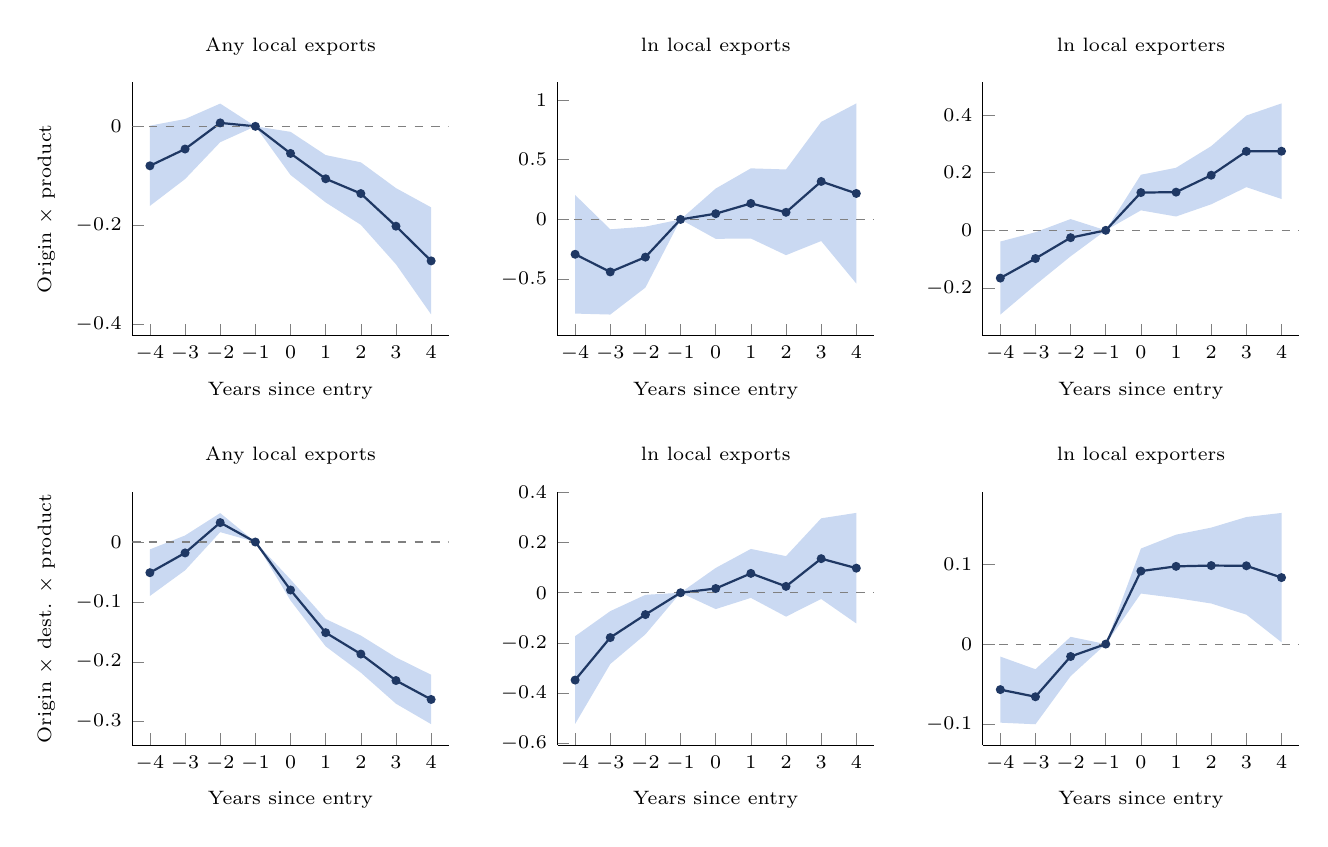
\begin{tikzpicture}
\begin{axis}[xshift=0.0cm, yshift=0.0cm, width=5.6cm, height=4.8cm, xmin=-4.5, xmax=4.5, ymin=-0.423, ymax=0.089,
  xtick={-4,-3,-2,-1,0,1,2,3,4}, tick label style={font=\scriptsize}, title={Any local exports}, title style={font=\scriptsize},
  xlabel={Years since entry}, xlabel style={font=\scriptsize}, axis x line*=bottom, axis y line*=left, ylabel={Origin $\times$ product}, ylabel style={font=\scriptsize}]
\addplot[draw=none, fill={rgb,255:red,166;green,191;blue,233}, fill opacity=0.6] coordinates {(-4,-0.1608) (-3,-0.1066) (-2,-0.0321) (-1,0.0000) (0,-0.0983) (1,-0.1538) (2,-0.1991) (3,-0.2788) (4,-0.3801) (4,-0.1638) (3,-0.1249) (2,-0.0728) (1,-0.0581) (0,-0.0112) (-1,0.0000) (-2,0.0459) (-3,0.0147) (-4,0.0013)} -- cycle;
\addplot[thick, mark=*, mark size=1.2pt, color={rgb,255:red,31;green,56;blue,100}] coordinates {(-4,-0.0798) (-3,-0.0459) (-2,0.0069) (-1,0.0000) (0,-0.0548) (1,-0.1060) (2,-0.1359) (3,-0.2018) (4,-0.2719)};
\draw[gray, dashed] (axis cs:-4.5,0) -- (axis cs:4.5,0);
\end{axis}
\begin{axis}[xshift=5.4cm, yshift=0.0cm, width=5.6cm, height=4.8cm, xmin=-4.5, xmax=4.5, ymin=-0.972, ymax=1.147,
  xtick={-4,-3,-2,-1,0,1,2,3,4}, tick label style={font=\scriptsize}, title={$\ln$ local exports}, title style={font=\scriptsize},
  xlabel={Years since entry}, xlabel style={font=\scriptsize}, axis x line*=bottom, axis y line*=left]
\addplot[draw=none, fill={rgb,255:red,166;green,191;blue,233}, fill opacity=0.6] coordinates {(-4,-0.7873) (-3,-0.7953) (-2,-0.5700) (-1,0.0000) (0,-0.1623) (1,-0.1595) (2,-0.2987) (3,-0.1807) (4,-0.5361) (4,0.9701) (3,0.8154) (2,0.4177) (1,0.4269) (0,0.2582) (-1,0.0000) (-2,-0.0604) (-3,-0.0826) (-4,0.2045)} -- cycle;
\addplot[thick, mark=*, mark size=1.2pt, color={rgb,255:red,31;green,56;blue,100}] coordinates {(-4,-0.2914) (-3,-0.4390) (-2,-0.3152) (-1,0.0000) (0,0.0480) (1,0.1337) (2,0.0595) (3,0.3174) (4,0.2170)};
\draw[gray, dashed] (axis cs:-4.5,0) -- (axis cs:4.5,0);
\end{axis}
\begin{axis}[xshift=10.8cm, yshift=0.0cm, width=5.6cm, height=4.8cm, xmin=-4.5, xmax=4.5, ymin=-0.365, ymax=0.513,
  xtick={-4,-3,-2,-1,0,1,2,3,4}, tick label style={font=\scriptsize}, title={$\ln$ local exporters}, title style={font=\scriptsize},
  xlabel={Years since entry}, xlabel style={font=\scriptsize}, axis x line*=bottom, axis y line*=left]
\addplot[draw=none, fill={rgb,255:red,166;green,191;blue,233}, fill opacity=0.6] coordinates {(-4,-0.2921) (-3,-0.1889) (-2,-0.0901) (-1,0.0000) (0,0.0692) (1,0.0479) (2,0.0902) (3,0.1495) (4,0.1085) (4,0.4397) (3,0.3978) (2,0.2917) (1,0.2168) (0,0.1925) (-1,0.0000) (-2,0.0390) (-3,-0.0066) (-4,-0.0389)} -- cycle;
\addplot[thick, mark=*, mark size=1.2pt, color={rgb,255:red,31;green,56;blue,100}] coordinates {(-4,-0.1655) (-3,-0.0977) (-2,-0.0255) (-1,0.0000) (0,0.1308) (1,0.1323) (2,0.1909) (3,0.2736) (4,0.2741)};
\draw[gray, dashed] (axis cs:-4.5,0) -- (axis cs:4.5,0);
\end{axis}
\begin{axis}[xshift=0.0cm, yshift=-5.2cm, width=5.6cm, height=4.8cm, xmin=-4.5, xmax=4.5, ymin=-0.339, ymax=0.084,
  xtick={-4,-3,-2,-1,0,1,2,3,4}, tick label style={font=\scriptsize}, title={Any local exports}, title style={font=\scriptsize},
  xlabel={Years since entry}, xlabel style={font=\scriptsize}, axis x line*=bottom, axis y line*=left, ylabel={Origin $\times$ dest. $\times$ product}, ylabel style={font=\scriptsize}]
\addplot[draw=none, fill={rgb,255:red,166;green,191;blue,233}, fill opacity=0.6] coordinates {(-4,-0.0900) (-3,-0.0473) (-2,0.0165) (-1,0.0000) (0,-0.0976) (1,-0.1742) (2,-0.2180) (3,-0.2699) (4,-0.3040) (4,-0.2216) (3,-0.1926) (2,-0.1561) (1,-0.1285) (0,-0.0625) (-1,0.0000) (-2,0.0483) (-3,0.0109) (-4,-0.0123)} -- cycle;
\addplot[thick, mark=*, mark size=1.2pt, color={rgb,255:red,31;green,56;blue,100}] coordinates {(-4,-0.0512) (-3,-0.0182) (-2,0.0324) (-1,0.0000) (0,-0.0801) (1,-0.1513) (2,-0.1870) (3,-0.2312) (4,-0.2628)};
\draw[gray, dashed] (axis cs:-4.5,0) -- (axis cs:4.5,0);
\end{axis}
\begin{axis}[xshift=5.4cm, yshift=-5.2cm, width=5.6cm, height=4.8cm, xmin=-4.5, xmax=4.5, ymin=-0.606, ymax=0.402,
  xtick={-4,-3,-2,-1,0,1,2,3,4}, tick label style={font=\scriptsize}, title={$\ln$ local exports}, title style={font=\scriptsize},
  xlabel={Years since entry}, xlabel style={font=\scriptsize}, axis x line*=bottom, axis y line*=left]
\addplot[draw=none, fill={rgb,255:red,166;green,191;blue,233}, fill opacity=0.6] coordinates {(-4,-0.5217) (-3,-0.2835) (-2,-0.1654) (-1,0.0000) (0,-0.0649) (1,-0.0204) (2,-0.0949) (3,-0.0248) (4,-0.1221) (4,0.3177) (3,0.2961) (2,0.1457) (1,0.1743) (0,0.0987) (-1,0.0000) (-2,-0.0083) (-3,-0.0732) (-4,-0.1728)} -- cycle;
\addplot[thick, mark=*, mark size=1.2pt, color={rgb,255:red,31;green,56;blue,100}] coordinates {(-4,-0.3473) (-3,-0.1783) (-2,-0.0868) (-1,0.0000) (0,0.0169) (1,0.0770) (2,0.0254) (3,0.1356) (4,0.0978)};
\draw[gray, dashed] (axis cs:-4.5,0) -- (axis cs:4.5,0);
\end{axis}
\begin{axis}[xshift=10.8cm, yshift=-5.2cm, width=5.6cm, height=4.8cm, xmin=-4.5, xmax=4.5, ymin=-0.126, ymax=0.190,
  xtick={-4,-3,-2,-1,0,1,2,3,4}, tick label style={font=\scriptsize}, title={$\ln$ local exporters}, title style={font=\scriptsize},
  xlabel={Years since entry}, xlabel style={font=\scriptsize}, axis x line*=bottom, axis y line*=left]
\addplot[draw=none, fill={rgb,255:red,166;green,191;blue,233}, fill opacity=0.6] coordinates {(-4,-0.0980) (-3,-0.1000) (-2,-0.0400) (-1,0.0000) (0,0.0630) (1,0.0574) (2,0.0506) (3,0.0367) (4,0.0023) (4,0.1635) (3,0.1584) (2,0.1452) (1,0.1364) (0,0.1191) (-1,0.0000) (-2,0.0090) (-3,-0.0314) (-4,-0.0156)} -- cycle;
\addplot[thick, mark=*, mark size=1.2pt, color={rgb,255:red,31;green,56;blue,100}] coordinates {(-4,-0.0568) (-3,-0.0657) (-2,-0.0155) (-1,0.0000) (0,0.0910) (1,0.0969) (2,0.0979) (3,0.0976) (4,0.0829)};
\draw[gray, dashed] (axis cs:-4.5,0) -- (axis cs:4.5,0);
\end{axis}
\end{tikzpicture}}
{The figure shows the Callaway and Sant'Anna (2021) estimates by year since entry, relative to the year before entry,
with 95 percent confidence intervals. Top row: origin $\times$ product cells. Bottom row: origin $\times$ destination
$\times$ product cells.}{\srcnote}

\FloatBarrier
\section{Conclusions}\label{sec:conclusions}

We have used firm level customs data from nine Latin American countries, linked to ownership data, to show that
multinational firms ship almost half of the agricultural exports of the region, less than in mining and manufacturing.
Their parents are concentrated in a few countries, a quarter of their exports comes from groups registered in
jurisdictions such as Switzerland and Liechtenstein, and twenty groups ship half of the exports of foreign affiliates.

We have then shown that exports are larger where more multinationals export the same product to the same destination,
and so are the exports of local firms. Capital intensity organizes part of this association. It is stronger for farm
products with high capital intensity, mainly grains and oilseeds, and it does not differ in a robust way among
processed products. Multinationals are not more likely to export capital intensive products, so the stronger
association is not a matter of where they choose to be. We have finally shown that fewer markets keep local exports
after the first multinational enters a product or a market, but local exports were already growing before entry.

These patterns are associations. Measuring the effect of multinational presence on the exports of local firms would
require changes in presence that are not related to the conditions of each market. Investment promotion, which shifts
where multinationals locate (Carballo, Marra de Arti\~nano and Volpe Martincus, 2026), is a natural source of such
changes and a promising avenue for future research.

\section*{References}

{\sloppy
\begin{list}{}{\leftmargin=1.5em \itemindent=-1.5em \itemsep=2pt \topsep=4pt}
\item Aitken, B., Hanson, G.\ H.\ and Harrison, A.\ E., 1997. Spillovers, Foreign Investment, and Export Behavior. \emph{Journal of International Economics}, 43(1), 103 to 132.
\item Becker, R.\ A., Gray, W.\ B.\ and Marvakov, J., 2021. NBER and CES Manufacturing Industry Database (1958 to 2018, version 2021a). Cambridge, MA: National Bureau of Economic Research.
\item Callaway, B.\ and Sant'Anna, P.\ H.\ C., 2021. Difference in Differences with Multiple Time Periods. \emph{Journal of Econometrics}, 225(2), 200 to 230.
\item Carballo, J., Marra de Arti\~nano, I.\ and Volpe Martincus, C., 2026. The Impact of Investment Promotion on Multinational Production: Firm Level Evidence. \emph{Journal of Development Economics}, 180.
\item Carballo, J., Marra de Arti\~nano, I., Ottaviano, G.\ I.\ P.\ and Volpe Martincus, C., 2021. Linkages with Multinationals: The Effects on Domestic Firms' Exports. Mimeo, Inter-American Development Bank.
\item Clapp, J., 2015. ABCD and Beyond: From Grain Merchants to Agricultural Value Chain Managers. \emph{Canadian Food Studies}, 2(2), 126 to 135.
\item Correia, S., Guimar\~aes, P.\ and Zylkin, T., 2020. Fast Poisson Estimation with High Dimensional Fixed Effects. \emph{Stata Journal}, 20(1), 95 to 115.
\item FAO, 2015. \emph{World Programme for the Census of Agriculture 2020, Volume 1: Programme, Concepts and Definitions}. FAO Statistical Development Series 15. Rome: Food and Agriculture Organization of the United Nations.
\item Javorcik, B.\ S., 2004. Does Foreign Direct Investment Increase the Productivity of Domestic Firms? In Search of Spillovers through Backward Linkages. \emph{American Economic Review}, 94(3), 605 to 627.
\item Murphy, S., Burch, D.\ and Clapp, J., 2012. \emph{Cereal Secrets: The World's Largest Grain Traders and Global Agriculture}. Oxfam Research Reports. Oxford: Oxfam International.
\item Rauch, J.\ E., 1999. Networks versus Markets in International Trade. \emph{Journal of International Economics}, 48(1), 7 to 35.
\item Reardon, T., Barrett, C.\ B., Berdegu\'e, J.\ A.\ and Swinnen, J.\ F.\ M., 2009. Agrifood Industry Transformation and Small Farmers in Developing Countries. \emph{World Development}, 37(11), 1717 to 1727.
\item Sun, L.\ and Abraham, S., 2021. Estimating Dynamic Treatment Effects in Event Studies with Heterogeneous Treatment Effects. \emph{Journal of Econometrics}, 225(2), 175 to 199.
\item UNCTAD, 2009. \emph{World Investment Report 2009: Transnational Corporations, Agricultural Production and Development}. New York and Geneva: United Nations.
\item UNSD, 2026. Correspondence tables between HS 2017, HS 2012, HS 2007, CPC Ver. 2.1, ISIC Rev. 4 and NAICS 2017. United Nations Statistics Division, Classifications on Economic Statistics. Accessed 3 November 2026.
\item USDA NASS, 2019. \emph{2017 Census of Agriculture: United States Summary and State Data}, Volume 1, Geographic Area Series, Part 51. Washington, DC: US Department of Agriculture, National Agricultural Statistics Service.
\end{list}
}

\clearpage
\appendix
\setcounter{table}{0}\renewcommand{\thetable}{A.\arabic{table}}
\setcounter{figure}{0}\renewcommand{\thefigure}{A.\arabic{figure}}
\section*{Appendix}

The workbook that accompanies this paper reports every estimate, with all the fixed effects, samples and tests. This
appendix reports the versions with the exports of local firms, with the indicator for at least one multinational as the
regressor, by country, and the secondary crosses.

\subsection*{Exports of local firms}

\vtab{tab:a_local}{Multinational presence and the agricultural exports of local firms}{\begin{tabular}{l*{6}{c}}
\toprule
 & (1) & (2) & (3) & (4) & (5) & (6) \\
\midrule
\multicolumn{7}{l}{\textit{Panel A. Intensive margin: cells with at least one MNE}} \\
$\ln$(number of MNEs) & 1.565*** & 1.576*** & 0.410*** & 0.373*** & 0.298*** & 0.179*** \\
 & (0.036) & (0.036) & (0.029) & (0.028) & (0.028) & (0.049) \\
Observations (Panel A) & 60,048 & 59,912 & 54,568 & 52,846 & 48,572 & 18,104 \\
$R^2$ & 0.491 & 0.501 & 0.878 & 0.891 & 0.914 & 0.967 \\
\midrule
\multicolumn{7}{l}{\textit{Panel B. Extensive margin: all cells}} \\
At least one MNE & 1.951*** & 1.951*** & 0.261*** & 0.237*** & 0.187*** & 0.093*** \\
 & (0.063) & (0.062) & (0.022) & (0.021) & (0.020) & (0.032) \\
Observations (Panel B) & 156,896 & 156,829 & 139,183 & 137,470 & 130,977 & 62,726 \\
$R^2$ & 0.419 & 0.429 & 0.866 & 0.875 & 0.898 & 0.947 \\
\midrule
Origin FE & $\checkmark$ &  &  &  &  &  \\
Destination FE & $\checkmark$ &  &  &  &  &  \\
Product FE & $\checkmark$ & $\checkmark$ &  &  &  &  \\
Year FE & $\checkmark$ &  & $\checkmark$ &  &  &  \\
Origin $\times$ year FE &  & $\checkmark$ &  &  &  &  \\
Destination $\times$ year FE &  & $\checkmark$ &  &  &  &  \\
Origin $\times$ destination $\times$ product FE &  &  & $\checkmark$ & $\checkmark$ & $\checkmark$ & $\checkmark$ \\
Origin $\times$ destination $\times$ year FE &  &  &  & $\checkmark$ & $\checkmark$ & $\checkmark$ \\
Origin $\times$ product $\times$ year FE &  &  &  &  & $\checkmark$ & $\checkmark$ \\
Destination $\times$ product $\times$ year FE &  &  &  &  &  & $\checkmark$ \\
\bottomrule
\end{tabular}}
{The table reports estimated coefficients of equation~(\ref{eq:presence}). The dependent variable is the natural
logarithm of the exports of local firms, on cells with positive local exports. Standard errors clustered by pair of
origin and destination countries are reported in parentheses. \SIG}{\srcnote}

\vtab{tab:a_zeros}{Multinational presence and the probability of local exports}{\begin{tabular}{l*{4}{c}}
\toprule
 & (1) & (2) & (3) & (4) \\
\midrule
\multicolumn{5}{l}{\textit{Panel A. Positive local exports, cells with at least one MNE}} \\
$\ln$(number of MNEs) & 0.043*** & 0.035*** & 0.024*** & 0.013* \\
 & (0.004) & (0.004) & (0.004) & (0.007) \\
Observations (Panel A) & 90,311 & 88,525 & 82,787 & 32,982 \\
$R^2$ & 0.736 & 0.763 & 0.806 & 0.907 \\
\midrule
\multicolumn{5}{l}{\textit{Panel B. Positive local exports, all cells}} \\
At least one MNE & -0.300*** & -0.294*** & -0.277*** & -0.235*** \\
 & (0.007) & (0.007) & (0.006) & (0.007) \\
Observations (Panel B) & 177,873 & 176,192 & 169,531 & 90,414 \\
$R^2$ & 0.732 & 0.750 & 0.783 & 0.874 \\
\midrule
Year FE & $\checkmark$ &  &  &  \\
Origin $\times$ destination $\times$ product FE & $\checkmark$ & $\checkmark$ & $\checkmark$ & $\checkmark$ \\
Origin $\times$ destination $\times$ year FE &  & $\checkmark$ & $\checkmark$ & $\checkmark$ \\
Origin $\times$ product $\times$ year FE &  &  & $\checkmark$ & $\checkmark$ \\
Destination $\times$ product $\times$ year FE &  &  &  & $\checkmark$ \\
\bottomrule
\end{tabular}}
{The table reports estimated coefficients of linear probability models. The dependent variable is an indicator for
positive local exports, on all cells with exports, including cells with no local exports. Columns 1 to 4 have the fixed
effects of columns 3 to 6 of Table~\ref{tab:base}. In Panel B the comparison is mechanical: a cell without an MNE has
local exports by definition. PPML on local exports in levels with the fixed effects of column 2 gives an elasticity of
0.53 (standard error 0.06) with the natural logarithm of the number of MNEs and a coefficient of 0.20 (0.05) on the
indicator. Standard errors clustered by pair of origin and destination countries are reported in parentheses. \SIG}{\srcnote}

\vtab{tab:a_exporters}{Multinational presence, the number of local exporters and exports per local exporter}{\begin{tabular}{l*{4}{c}}
\toprule
 & (1) & (2) & (3) & (4) \\
\midrule
\multicolumn{5}{l}{\textit{Panel A. $\ln$ number of local exporters}} \\
$\ln$(number of MNEs) & 0.246*** & 0.227*** & 0.182*** & 0.119*** \\
 & (0.012) & (0.012) & (0.011) & (0.017) \\
Observations (Panel A) & 54,568 & 52,846 & 48,572 & 18,104 \\
$R^2$ & 0.878 & 0.894 & 0.920 & 0.975 \\
\midrule
\multicolumn{5}{l}{\textit{Panel B. $\ln$ exports per local exporter}} \\
$\ln$(number of MNEs) & 0.164*** & 0.146*** & 0.116*** & 0.060 \\
 & (0.021) & (0.020) & (0.021) & (0.042) \\
Observations (Panel B) & 54,568 & 52,846 & 48,572 & 18,104 \\
$R^2$ & 0.863 & 0.876 & 0.900 & 0.957 \\
\midrule
\multicolumn{5}{l}{\textit{Panel C. $\ln$ number of local exporters}} \\
At least one MNE & 0.140*** & 0.126*** & 0.102*** & 0.058*** \\
 & (0.008) & (0.007) & (0.007) & (0.009) \\
Observations (Panel C) & 139,183 & 137,470 & 130,977 & 62,726 \\
$R^2$ & 0.846 & 0.861 & 0.888 & 0.954 \\
\midrule
\multicolumn{5}{l}{\textit{Panel D. $\ln$ exports per local exporter}} \\
At least one MNE & 0.121*** & 0.111*** & 0.085*** & 0.035 \\
 & (0.018) & (0.018) & (0.018) & (0.031) \\
Observations (Panel D) & 139,183 & 137,470 & 130,977 & 62,726 \\
$R^2$ & 0.854 & 0.863 & 0.887 & 0.937 \\
\midrule
Year FE & $\checkmark$ &  &  &  \\
Origin $\times$ destination $\times$ product FE & $\checkmark$ & $\checkmark$ & $\checkmark$ & $\checkmark$ \\
Origin $\times$ destination $\times$ year FE &  & $\checkmark$ & $\checkmark$ & $\checkmark$ \\
Origin $\times$ product $\times$ year FE &  &  & $\checkmark$ & $\checkmark$ \\
Destination $\times$ product $\times$ year FE &  &  &  & $\checkmark$ \\
\bottomrule
\end{tabular}}
{The table reports estimated coefficients of equation~(\ref{eq:presence}) on cells with at least one local exporter.
The dependent variables are the natural logarithms of the number of local exporters and of exports per local exporter.
Panels A and B: natural logarithm of the number of MNEs, cells with at least one MNE. Panels C and D: indicator for at
least one MNE. Columns 1 to 4 have the fixed effects of columns 3 to 6 of Table~\ref{tab:base}. Standard errors
clustered by pair of origin and destination countries are reported in parentheses. \SIG}{\srcnote}

\vtab{tab:a_hetlocal}{Multinational presence and the exports of local firms, by capital intensity}{\begin{tabular}{l*{4}{c}}
\toprule
 & (1) & (2) & (3) & (4) \\
\midrule
\multicolumn{5}{l}{\textit{Panel A. Stages pooled, aggregate ratio}} \\
$\ln$(number of MNEs) $\times$ high capital intensity & 0.372*** & 0.336*** & 0.287*** & 0.074 \\
 & (0.036) & (0.035) & (0.038) & (0.083) \\
$\ln$(number of MNEs) $\times$ low capital intensity & 0.442*** & 0.404*** & 0.306*** & 0.259*** \\
 & (0.036) & (0.035) & (0.031) & (0.058) \\
$\ln$(number of MNEs) $\times$ not classified & 0.540*** & 0.550*** & 0.372** & 0.403 \\
 & (0.142) & (0.155) & (0.187) & (0.500) \\
$p$ value: high = low & 0.099 & 0.105 & 0.654 & 0.063 \\
Observations (Panel A) & 54,568 & 52,846 & 48,572 & 18,104 \\
$R^2$ & 0.878 & 0.891 & 0.914 & 0.967 \\
\midrule
\multicolumn{5}{l}{\textit{Panel B. Stages pooled, median}} \\
$\ln$(number of MNEs) $\times$ high capital intensity & 0.518*** & 0.500*** & 0.410*** & 0.167 \\
 & (0.049) & (0.051) & (0.064) & (0.147) \\
$\ln$(number of MNEs) $\times$ low capital intensity & 0.380*** & 0.336*** & 0.268*** & 0.180*** \\
 & (0.032) & (0.031) & (0.028) & (0.052) \\
$\ln$(number of MNEs) $\times$ not classified & 0.540*** & 0.550*** & 0.371** & 0.388 \\
 & (0.142) & (0.154) & (0.187) & (0.492) \\
$p$ value: high = low & 0.011 & 0.004 & 0.033 & 0.934 \\
Observations (Panel B) & 54,568 & 52,846 & 48,572 & 18,104 \\
$R^2$ & 0.878 & 0.891 & 0.914 & 0.967 \\
\midrule
\multicolumn{5}{l}{\textit{Panel C. By stage, aggregate ratio}} \\
$\ln$(number of MNEs) $\times$ farm stage, high & 0.708*** & 0.692*** & 0.589*** & 0.494** \\
 & (0.067) & (0.070) & (0.090) & (0.225) \\
$\ln$(number of MNEs) $\times$ farm stage, low & 0.394*** & 0.341*** & 0.247*** & 0.249*** \\
 & (0.045) & (0.040) & (0.038) & (0.074) \\
$\ln$(number of MNEs) $\times$ processing stage, high & 0.274*** & 0.234*** & 0.197*** & 0.036 \\
 & (0.038) & (0.037) & (0.037) & (0.086) \\
$\ln$(number of MNEs) $\times$ processing stage, low & 0.517*** & 0.496*** & 0.398*** & 0.273*** \\
 & (0.048) & (0.051) & (0.047) & (0.094) \\
$\ln$(number of MNEs) $\times$ not classified & 0.541*** & 0.547*** & 0.372** & 0.334 \\
 & (0.142) & (0.154) & (0.187) & (0.495) \\
$p$ value: farm stage, high = low & 0.000 & 0.000 & 0.000 & 0.316 \\
$p$ value: processing stage, high = low & 0.000 & 0.000 & 0.000 & 0.067 \\
Observations (Panel C) & 54,568 & 52,846 & 48,572 & 18,104 \\
$R^2$ & 0.878 & 0.891 & 0.914 & 0.967 \\
\midrule
Year FE & $\checkmark$ &  &  &  \\
Origin $\times$ destination $\times$ product FE & $\checkmark$ & $\checkmark$ & $\checkmark$ & $\checkmark$ \\
Origin $\times$ destination $\times$ year FE &  & $\checkmark$ & $\checkmark$ & $\checkmark$ \\
Origin $\times$ product $\times$ year FE &  &  & $\checkmark$ & $\checkmark$ \\
Destination $\times$ product $\times$ year FE &  &  &  & $\checkmark$ \\
\bottomrule
\end{tabular}}
{The table reports estimates as in Table~\ref{tab:het}. The dependent variable is the natural logarithm of the exports
of local firms. Standard errors clustered by pair of origin and destination countries are reported in parentheses.
\SIG}{\srcnote}

\clearpage
\subsection*{Indicator for at least one multinational}

\vtab{tab:a_hetD}{At least one multinational and agricultural exports, by capital intensity}{\begin{tabular}{l*{4}{c}}
\toprule
 & (1) & (2) & (3) & (4) \\
\midrule
\multicolumn{5}{l}{\textit{Panel A. Stages pooled, aggregate ratio}} \\
At least one MNE $\times$ high capital intensity & 0.686*** & 0.681*** & 0.647*** & 0.640*** \\
 & (0.034) & (0.033) & (0.032) & (0.046) \\
At least one MNE $\times$ low capital intensity & 0.648*** & 0.638*** & 0.583*** & 0.510*** \\
 & (0.035) & (0.034) & (0.031) & (0.046) \\
At least one MNE $\times$ not classified & 0.288* & 0.350** & 0.508*** & -0.040 \\
 & (0.169) & (0.171) & (0.160) & (0.234) \\
$p$ value: high = low & 0.352 & 0.283 & 0.088 & 0.018 \\
Observations (Panel A) & 177,873 & 176,192 & 169,531 & 90,414 \\
$R^2$ & 0.870 & 0.878 & 0.899 & 0.946 \\
\midrule
\multicolumn{5}{l}{\textit{Panel B. Stages pooled, median}} \\
At least one MNE $\times$ high capital intensity & 0.813*** & 0.810*** & 0.746*** & 0.761*** \\
 & (0.046) & (0.047) & (0.045) & (0.075) \\
At least one MNE $\times$ low capital intensity & 0.630*** & 0.622*** & 0.584*** & 0.542*** \\
 & (0.031) & (0.029) & (0.027) & (0.039) \\
At least one MNE $\times$ not classified & 0.288* & 0.349** & 0.508*** & -0.038 \\
 & (0.169) & (0.171) & (0.160) & (0.233) \\
$p$ value: high = low & 0.000 & 0.000 & 0.000 & 0.007 \\
Observations (Panel B) & 177,873 & 176,192 & 169,531 & 90,414 \\
$R^2$ & 0.870 & 0.878 & 0.899 & 0.946 \\
\midrule
\multicolumn{5}{l}{\textit{Panel C. By stage, aggregate ratio}} \\
At least one MNE $\times$ farm stage, high & 0.870*** & 0.872*** & 0.743*** & 0.718*** \\
 & (0.066) & (0.067) & (0.068) & (0.127) \\
At least one MNE $\times$ farm stage, low & 0.667*** & 0.654*** & 0.601*** & 0.517*** \\
 & (0.041) & (0.039) & (0.037) & (0.055) \\
At least one MNE $\times$ processing stage, high & 0.653*** & 0.648*** & 0.630*** & 0.632*** \\
 & (0.038) & (0.037) & (0.036) & (0.048) \\
At least one MNE $\times$ processing stage, low & 0.622*** & 0.615*** & 0.558*** & 0.501*** \\
 & (0.046) & (0.047) & (0.044) & (0.068) \\
At least one MNE $\times$ not classified & 0.288* & 0.350** & 0.508*** & -0.040 \\
 & (0.169) & (0.171) & (0.160) & (0.234) \\
$p$ value: farm stage, high = low & 0.007 & 0.004 & 0.055 & 0.147 \\
$p$ value: processing stage, high = low & 0.547 & 0.545 & 0.165 & 0.072 \\
Observations (Panel C) & 177,873 & 176,192 & 169,531 & 90,414 \\
$R^2$ & 0.870 & 0.878 & 0.899 & 0.946 \\
\midrule
Year FE & $\checkmark$ &  &  &  \\
Origin $\times$ destination $\times$ product FE & $\checkmark$ & $\checkmark$ & $\checkmark$ & $\checkmark$ \\
Origin $\times$ destination $\times$ year FE &  & $\checkmark$ & $\checkmark$ & $\checkmark$ \\
Origin $\times$ product $\times$ year FE &  &  & $\checkmark$ & $\checkmark$ \\
Destination $\times$ product $\times$ year FE &  &  &  & $\checkmark$ \\
\bottomrule
\end{tabular}}
{The table reports estimates as in Table~\ref{tab:het} with the indicator for at least one MNE in place of the natural
logarithm of the number of MNEs, on all cells. Standard errors clustered by pair of origin and destination countries are
reported in parentheses. \SIG}{\srcnote}

\clearpage
\subsection*{By country}

\vtab{tab:a_country}{Multinational presence and agricultural exports, by exporting country}{\begin{tabular}{l*{9}{c}}
\toprule
 & ARG & PER & CHL & COL & PRY & URY & CRI & DOM & SLV \\
\midrule
\multicolumn{10}{l}{\textit{Panel A. Destination $\times$ product and year FE}} \\
$\ln$(number of MNEs) & 0.880*** & 0.953*** & 0.765*** & 0.744*** & 0.921*** & 1.060*** & 0.643*** & 0.506*** & 0.552*** \\
 & (0.041) & (0.057) & (0.032) & (0.055) & (0.082) & (0.086) & (0.097) & (0.055) & (0.133) \\
Observations (Panel A) & 21,108 & 13,199 & 19,135 & 10,864 & 2,512 & 5,340 & 7,781 & 6,882 & 3,490 \\
$R^2$ & 0.908 & 0.892 & 0.905 & 0.897 & 0.932 & 0.922 & 0.871 & 0.875 & 0.941 \\
\midrule
\multicolumn{10}{l}{\textit{Panel B. Destination $\times$ product and destination $\times$ year FE}} \\
$\ln$(number of MNEs) & 0.855*** & 0.934*** & 0.733*** & 0.719*** & 0.863*** & 0.994*** & 0.596*** & 0.574*** & 0.616*** \\
 & (0.041) & (0.053) & (0.031) & (0.055) & (0.095) & (0.095) & (0.100) & (0.053) & (0.139) \\
Observations (Panel B) & 20,957 & 12,998 & 18,904 & 10,638 & 2,274 & 5,111 & 7,597 & 6,672 & 3,374 \\
$R^2$ & 0.913 & 0.901 & 0.911 & 0.906 & 0.946 & 0.934 & 0.888 & 0.893 & 0.951 \\
\midrule
\multicolumn{10}{l}{\textit{Panel C. Panel B plus product $\times$ year FE}} \\
$\ln$(number of MNEs) & 0.792*** & 0.721*** & 0.656*** & 0.598*** & 0.685*** & 1.034*** & 0.520*** & 0.530*** & 0.452*** \\
 & (0.044) & (0.050) & (0.032) & (0.067) & (0.113) & (0.068) & (0.073) & (0.078) & (0.152) \\
Observations (Panel C) & 20,323 & 12,396 & 18,232 & 9,901 & 1,986 & 4,417 & 6,920 & 5,988 & 2,624 \\
$R^2$ & 0.926 & 0.923 & 0.928 & 0.924 & 0.963 & 0.938 & 0.920 & 0.924 & 0.965 \\
\midrule
Year FE (Panel A) & $\checkmark$ & $\checkmark$ & $\checkmark$ & $\checkmark$ & $\checkmark$ & $\checkmark$ & $\checkmark$ & $\checkmark$ & $\checkmark$ \\
Destination $\times$ product FE & $\checkmark$ & $\checkmark$ & $\checkmark$ & $\checkmark$ & $\checkmark$ & $\checkmark$ & $\checkmark$ & $\checkmark$ & $\checkmark$ \\
Destination $\times$ year FE (Panel B, C) & $\checkmark$ & $\checkmark$ & $\checkmark$ & $\checkmark$ & $\checkmark$ & $\checkmark$ & $\checkmark$ & $\checkmark$ & $\checkmark$ \\
Product $\times$ year FE (Panel C) & $\checkmark$ & $\checkmark$ & $\checkmark$ & $\checkmark$ & $\checkmark$ & $\checkmark$ & $\checkmark$ & $\checkmark$ & $\checkmark$ \\
\bottomrule
\end{tabular}}
{The table reports estimated coefficients of equation~(\ref{eq:presence}) for each exporting country (ISO 3166 codes),
on cells with at least one MNE. Within one country the origin dimension of each fixed effect is constant. Standard
errors clustered by destination country are reported in parentheses. \SIG}{\srcnote}

\vtab{tab:a_countryD}{At least one multinational and agricultural exports, by exporting country}{\begin{tabular}{l*{9}{c}}
\toprule
 & ARG & PER & CHL & COL & PRY & URY & CRI & DOM & SLV \\
\midrule
\multicolumn{10}{l}{\textit{Panel A. Destination $\times$ product and year FE}} \\
At least one MNE & 0.673*** & 0.853*** & 0.452*** & 0.575*** & 0.639*** & 0.619*** & 0.560*** & 0.836*** & 0.291* \\
 & (0.033) & (0.066) & (0.039) & (0.066) & (0.094) & (0.078) & (0.093) & (0.112) & (0.148) \\
Observations (Panel A) & 36,466 & 27,679 & 28,525 & 21,854 & 4,916 & 9,200 & 17,596 & 23,050 & 8,587 \\
$R^2$ & 0.873 & 0.833 & 0.883 & 0.838 & 0.891 & 0.884 & 0.820 & 0.824 & 0.904 \\
\midrule
\multicolumn{10}{l}{\textit{Panel B. Destination $\times$ product and destination $\times$ year FE}} \\
At least one MNE & 0.659*** & 0.861*** & 0.425*** & 0.607*** & 0.600*** & 0.606*** & 0.561*** & 0.844*** & 0.339** \\
 & (0.033) & (0.059) & (0.036) & (0.067) & (0.102) & (0.077) & (0.097) & (0.102) & (0.148) \\
Observations (Panel B) & 36,370 & 27,536 & 28,313 & 21,683 & 4,679 & 8,960 & 17,369 & 22,856 & 8,426 \\
$R^2$ & 0.878 & 0.842 & 0.889 & 0.847 & 0.908 & 0.898 & 0.830 & 0.834 & 0.913 \\
\midrule
\multicolumn{10}{l}{\textit{Panel C. Panel B plus product $\times$ year FE}} \\
At least one MNE & 0.623*** & 0.760*** & 0.440*** & 0.572*** & 0.609*** & 0.552*** & 0.517*** & 0.806*** & 0.211 \\
 & (0.029) & (0.057) & (0.035) & (0.064) & (0.097) & (0.068) & (0.084) & (0.114) & (0.129) \\
Observations (Panel C) & 35,831 & 26,923 & 27,486 & 20,812 & 4,209 & 8,105 & 16,436 & 22,096 & 7,633 \\
$R^2$ & 0.894 & 0.869 & 0.907 & 0.874 & 0.931 & 0.907 & 0.865 & 0.865 & 0.940 \\
\midrule
Year FE (Panel A) & $\checkmark$ & $\checkmark$ & $\checkmark$ & $\checkmark$ & $\checkmark$ & $\checkmark$ & $\checkmark$ & $\checkmark$ & $\checkmark$ \\
Destination $\times$ product FE & $\checkmark$ & $\checkmark$ & $\checkmark$ & $\checkmark$ & $\checkmark$ & $\checkmark$ & $\checkmark$ & $\checkmark$ & $\checkmark$ \\
Destination $\times$ year FE (Panel B, C) & $\checkmark$ & $\checkmark$ & $\checkmark$ & $\checkmark$ & $\checkmark$ & $\checkmark$ & $\checkmark$ & $\checkmark$ & $\checkmark$ \\
Product $\times$ year FE (Panel C) & $\checkmark$ & $\checkmark$ & $\checkmark$ & $\checkmark$ & $\checkmark$ & $\checkmark$ & $\checkmark$ & $\checkmark$ & $\checkmark$ \\
\bottomrule
\end{tabular}}
{The table reports estimates as in Table~\ref{tab:a_country} with the indicator for at least one MNE, on all cells.
Standard errors clustered by destination country are reported in parentheses. \SIG}{\srcnote}

\vtab{tab:a_hetcountry}{Multinational presence and agricultural exports by capital intensity, by exporting country}{\begin{tabular}{l*{9}{c}}
\toprule
 & ARG & PER & CHL & COL & PRY & URY & CRI & DOM & SLV \\
\midrule
\multicolumn{10}{l}{\textit{Panel A. Threshold: aggregate ratio of the stage}} \\
$\ln$(number of MNEs) $\times$ high capital intensity & 0.928*** & 0.797*** & 0.699*** & 0.832*** & 0.959*** & 1.336*** & 0.679*** & 0.590*** & 0.729*** \\
 & (0.049) & (0.059) & (0.053) & (0.108) & (0.121) & (0.096) & (0.126) & (0.061) & (0.156) \\
$\ln$(number of MNEs) $\times$ low capital intensity & 0.731*** & 1.046*** & 0.755*** & 0.659*** & 0.710*** & 0.789*** & 0.405*** & 0.576*** & 0.276*** \\
 & (0.050) & (0.078) & (0.037) & (0.065) & (0.166) & (0.135) & (0.079) & (0.087) & (0.101) \\
$\ln$(number of MNEs) $\times$ not classified & 0.807*** & 0.843*** & 2.081*** & 0.149 & 0.973*** & 0.563 & 3.118*** & -0.345 &  \\
 & (0.124) & (0.318) & (0.536) & (0.476) & (0.166) & (0.481) & (0.437) & (0.483) &  \\
$p$ value: high = low & 0.000 & 0.012 & 0.389 & 0.193 & 0.190 & 0.000 & 0.014 & 0.893 & 0.002 \\
Observations (Panel A) & 20,957 & 12,998 & 18,904 & 10,638 & 2,274 & 5,111 & 7,597 & 6,672 & 3,374 \\
$R^2$ & 0.913 & 0.901 & 0.911 & 0.906 & 0.947 & 0.935 & 0.888 & 0.893 & 0.951 \\
\midrule
\multicolumn{10}{l}{\textit{Panel B. Threshold: export weighted median}} \\
$\ln$(number of MNEs) $\times$ high capital intensity & 1.082*** & 0.823*** & 1.040*** & 0.850*** & 1.015*** & 1.594*** & 0.216 & 0.653*** & 0.783*** \\
 & (0.063) & (0.061) & (0.128) & (0.152) & (0.151) & (0.119) & (0.287) & (0.130) & (0.227) \\
$\ln$(number of MNEs) $\times$ low capital intensity & 0.727*** & 0.958*** & 0.709*** & 0.704*** & 0.706*** & 0.777*** & 0.572*** & 0.561*** & 0.567*** \\
 & (0.038) & (0.059) & (0.030) & (0.051) & (0.139) & (0.115) & (0.090) & (0.065) & (0.132) \\
$\ln$(number of MNEs) $\times$ not classified & 0.805*** & 0.843*** & 2.082*** & 0.148 & 0.973*** & 0.562 & 3.122*** & -0.346 &  \\
 & (0.124) & (0.318) & (0.536) & (0.476) & (0.165) & (0.477) & (0.436) & (0.483) &  \\
$p$ value: high = low & 0.000 & 0.081 & 0.007 & 0.332 & 0.122 & 0.000 & 0.150 & 0.565 & 0.245 \\
Observations (Panel B) & 20,957 & 12,998 & 18,904 & 10,638 & 2,274 & 5,111 & 7,597 & 6,672 & 3,374 \\
$R^2$ & 0.914 & 0.901 & 0.911 & 0.906 & 0.947 & 0.935 & 0.888 & 0.893 & 0.951 \\
\midrule
Destination $\times$ product FE & $\checkmark$ & $\checkmark$ & $\checkmark$ & $\checkmark$ & $\checkmark$ & $\checkmark$ & $\checkmark$ & $\checkmark$ & $\checkmark$ \\
Destination $\times$ year FE & $\checkmark$ & $\checkmark$ & $\checkmark$ & $\checkmark$ & $\checkmark$ & $\checkmark$ & $\checkmark$ & $\checkmark$ & $\checkmark$ \\
\bottomrule
\end{tabular}}
{The table reports estimates as in Table~\ref{tab:het}, Panels A and B, for each exporting country, with destination
$\times$ product and destination $\times$ year fixed effects. Standard errors clustered by destination country are
reported in parentheses. \SIG}{\srcnote}

\clearpage
\subsection*{Secondary crosses}

\vtab{tab:a_cont}{Multinational presence and agricultural exports: continuous capital intensity}{\begin{tabular}{l*{4}{c}}
\toprule
 & (1) & (2) & (3) & (4) \\
\midrule
\multicolumn{5}{l}{\textit{Panel A. $\ln$ capital per worker}} \\
$\ln$(number of MNEs) & 0.475*** & 0.384*** & 0.266*** & 0.418** \\
 & (0.102) & (0.100) & (0.094) & (0.170) \\
$\ln$(number of MNEs) $\times$ $\ln$ capital per worker & 0.078*** & 0.090*** & 0.096*** & 0.030 \\
 & (0.022) & (0.022) & (0.022) & (0.038) \\
Observations (Panel A) & 88,858 & 87,076 & 81,578 & 32,828 \\
$R^2$ & 0.907 & 0.917 & 0.933 & 0.969 \\
\midrule
\multicolumn{5}{l}{\textit{Panel B. $\ln$ capital per worker, deviation from the mean of the stage}} \\
$\ln$(number of MNEs) & 0.833*** & 0.799*** & 0.708*** & 0.562*** \\
 & (0.023) & (0.022) & (0.022) & (0.032) \\
$\ln$(number of MNEs) $\times$ $\ln$ capital per worker (within stage) & 0.098*** & 0.111*** & 0.128*** & 0.065 \\
 & (0.026) & (0.026) & (0.027) & (0.044) \\
Observations (Panel B) & 88,858 & 87,076 & 81,578 & 32,828 \\
$R^2$ & 0.907 & 0.917 & 0.933 & 0.969 \\
\midrule
Year FE & $\checkmark$ &  &  &  \\
Origin $\times$ destination $\times$ product FE & $\checkmark$ & $\checkmark$ & $\checkmark$ & $\checkmark$ \\
Origin $\times$ destination $\times$ year FE &  & $\checkmark$ & $\checkmark$ & $\checkmark$ \\
Origin $\times$ product $\times$ year FE &  &  & $\checkmark$ & $\checkmark$ \\
Destination $\times$ product $\times$ year FE &  &  &  & $\checkmark$ \\
\bottomrule
\end{tabular}}
{The table reports estimates of equation~(\ref{eq:presence}) for classified products with the natural logarithm of the
number of MNEs and its interaction with the natural logarithm of capital per worker. Panel B uses the deviation of the
natural logarithm of capital per worker from the mean of its stage. Standard errors clustered by pair of origin and
destination countries are reported in parentheses. \SIG}{\srcnote}

\vtab{tab:a_type}{Multinational presence and agricultural exports, by type of production}{\begin{tabular}{l*{4}{c}}
\toprule
 & (1) & (2) & (3) & (4) \\
\midrule
\multicolumn{5}{l}{\textit{Panel A. Type of production}} \\
$\ln$(number of MNEs) $\times$ field crops & 1.037*** & 1.009*** & 0.931*** & 0.990*** \\
 & (0.043) & (0.044) & (0.052) & (0.101) \\
$\ln$(number of MNEs) $\times$ horticultural and plantation crops & 0.706*** & 0.673*** & 0.585*** & 0.485*** \\
 & (0.029) & (0.026) & (0.025) & (0.041) \\
$\ln$(number of MNEs) $\times$ livestock and fisheries & 0.957*** & 0.915*** & 0.812*** & 0.625*** \\
 & (0.036) & (0.038) & (0.036) & (0.065) \\
$\ln$(number of MNEs) $\times$ other processed food & 0.727*** & 0.705*** & 0.614*** & 0.469*** \\
 & (0.044) & (0.043) & (0.043) & (0.068) \\
$p$ value: field crops = horticultural & 0.000 & 0.000 & 0.000 & 0.000 \\
Observations (Panel A) & 90,311 & 88,525 & 82,787 & 32,982 \\
$R^2$ & 0.907 & 0.916 & 0.933 & 0.969 \\
\midrule
\multicolumn{5}{l}{\textit{Panel B. Type of production and capital intensity (aggregate ratio)}} \\
$\ln$(number of MNEs) $\times$ field crops, high & 1.070*** & 1.040*** & 0.947*** & 1.023*** \\
 & (0.046) & (0.047) & (0.055) & (0.101) \\
$\ln$(number of MNEs) $\times$ field crops, low & 0.495*** & 0.537*** & 0.538*** & 0.949** \\
 & (0.101) & (0.113) & (0.112) & (0.375) \\
$\ln$(number of MNEs) $\times$ horticultural and plantation, high & 0.704*** & 0.695*** & 0.613*** & 0.510*** \\
 & (0.036) & (0.034) & (0.035) & (0.069) \\
$\ln$(number of MNEs) $\times$ horticultural and plantation, low & 0.708*** & 0.658*** & 0.567*** & 0.466*** \\
 & (0.037) & (0.034) & (0.031) & (0.052) \\
$\ln$(number of MNEs) $\times$ livestock and fisheries, high & 0.927*** & 0.868*** & 0.818*** & 0.714*** \\
 & (0.065) & (0.066) & (0.072) & (0.150) \\
$\ln$(number of MNEs) $\times$ livestock and fisheries, low & 0.969*** & 0.930*** & 0.808*** & 0.600*** \\
 & (0.042) & (0.045) & (0.042) & (0.069) \\
$\ln$(number of MNEs) $\times$ other processed food, high & 0.718*** & 0.700*** & 0.611*** & 0.415*** \\
 & (0.046) & (0.048) & (0.048) & (0.080) \\
$\ln$(number of MNEs) $\times$ other processed food, low & 0.689*** & 0.649*** & 0.559*** & 0.606*** \\
 & (0.077) & (0.068) & (0.076) & (0.096) \\
$\ln$(number of MNEs) $\times$ not classified & 0.861*** & 0.874*** & 0.952*** & 0.005 \\
 & (0.140) & (0.143) & (0.153) & (0.516) \\
$p$ value: field crops, high = low & 0.000 & 0.000 & 0.001 & 0.852 \\
$p$ value: horticultural, high = low & 0.921 & 0.411 & 0.293 & 0.624 \\
$p$ value: livestock, high = low & 0.588 & 0.437 & 0.906 & 0.476 \\
$p$ value: other processed food, high = low & 0.700 & 0.488 & 0.520 & 0.085 \\
Observations (Panel B) & 90,311 & 88,525 & 82,787 & 32,982 \\
$R^2$ & 0.907 & 0.916 & 0.933 & 0.969 \\
\midrule
Year FE & $\checkmark$ &  &  &  \\
Origin $\times$ destination $\times$ product FE & $\checkmark$ & $\checkmark$ & $\checkmark$ & $\checkmark$ \\
Origin $\times$ destination $\times$ year FE &  & $\checkmark$ & $\checkmark$ & $\checkmark$ \\
Origin $\times$ product $\times$ year FE &  &  & $\checkmark$ & $\checkmark$ \\
Destination $\times$ product $\times$ year FE &  &  &  & $\checkmark$ \\
\bottomrule
\end{tabular}}
{The table reports estimates as in Table~\ref{tab:het} with the natural logarithm of the number of MNEs interacted with
the type of production (Panel A) and with the type of production and capital intensity (Panel B). Standard errors
clustered by pair of origin and destination countries are reported in parentheses. \SIG}{\srcnote}

\vtab{tab:a_cross}{Multinational presence and agricultural exports, by Rauch class, end use and inputs}{\begin{tabular}{l*{4}{c}}
\toprule
 & (1) & (2) & (3) & (4) \\
\midrule
\multicolumn{5}{l}{\textit{Panel A. Rauch (1999), conservative classification}} \\
$\ln$(number of MNEs) $\times$ homogeneous & 0.942*** & 0.897*** & 0.868*** & 0.732*** \\
 & (0.047) & (0.049) & (0.054) & (0.087) \\
$\ln$(number of MNEs) $\times$ reference priced & 0.804*** & 0.774*** & 0.659*** & 0.520*** \\
 & (0.026) & (0.025) & (0.023) & (0.041) \\
$\ln$(number of MNEs) $\times$ differentiated & 0.779*** & 0.752*** & 0.654*** & 0.507*** \\
 & (0.031) & (0.030) & (0.029) & (0.057) \\
$\ln$(number of MNEs) $\times$ not classified & 0.749*** & 0.894*** & 0.799*** & 0.652 \\
 & (0.133) & (0.163) & (0.181) & (0.399) \\
$p$ value: homogeneous = differentiated & 0.002 & 0.009 & 0.000 & 0.037 \\
Observations (Panel A) & 90,311 & 88,525 & 82,787 & 32,982 \\
$R^2$ & 0.907 & 0.916 & 0.933 & 0.969 \\
\midrule
\multicolumn{5}{l}{\textit{Panel B. BEC end use}} \\
$\ln$(number of MNEs) $\times$ intermediate goods & 0.873*** & 0.838*** & 0.780*** & 0.579*** \\
 & (0.037) & (0.039) & (0.045) & (0.057) \\
$\ln$(number of MNEs) $\times$ consumption goods & 0.810*** & 0.779*** & 0.675*** & 0.541*** \\
 & (0.025) & (0.024) & (0.021) & (0.035) \\
$p$ value: intermediate = consumption & 0.130 & 0.155 & 0.020 & 0.553 \\
Observations (Panel B) & 90,311 & 88,525 & 82,787 & 32,982 \\
$R^2$ & 0.907 & 0.916 & 0.933 & 0.969 \\
\midrule
\multicolumn{5}{l}{\textit{Panel C. Inputs}} \\
$\ln$(number of MNEs) $\times$ inputs & 0.937*** & 0.905*** & 0.788*** & 0.634*** \\
 & (0.057) & (0.059) & (0.057) & (0.092) \\
$\ln$(number of MNEs) $\times$ other products & 0.818*** & 0.785*** & 0.695*** & 0.543*** \\
 & (0.023) & (0.022) & (0.023) & (0.034) \\
$p$ value: inputs = other & 0.040 & 0.048 & 0.126 & 0.377 \\
Observations (Panel C) & 90,311 & 88,525 & 82,787 & 32,982 \\
$R^2$ & 0.907 & 0.916 & 0.932 & 0.969 \\
\midrule
Year FE & $\checkmark$ &  &  &  \\
Origin $\times$ destination $\times$ product FE & $\checkmark$ & $\checkmark$ & $\checkmark$ & $\checkmark$ \\
Origin $\times$ destination $\times$ year FE &  & $\checkmark$ & $\checkmark$ & $\checkmark$ \\
Origin $\times$ product $\times$ year FE &  &  & $\checkmark$ & $\checkmark$ \\
Destination $\times$ product $\times$ year FE &  &  &  & $\checkmark$ \\
\bottomrule
\end{tabular}}
{The table reports estimates as in Table~\ref{tab:het}. Rauch (1999), conservative classification, through the HS 2007
code of each HS 2017 product. End use from BEC Rev.4, with capital goods grouped with intermediate goods. Inputs: seeds,
animal feed and live animals. Standard errors clustered by pair of origin and destination countries are reported in
parentheses. \SIG}{\srcnote}

\vtab{tab:a_hetmed}{Multinational presence and agricultural exports, by capital intensity: median threshold}{\begin{tabular}{l*{4}{c}}
\toprule
 & (1) & (2) & (3) & (4) \\
\midrule
\multicolumn{5}{l}{\textit{Panel A. By stage}} \\
$\ln$(number of MNEs) $\times$ farm stage, high & 1.137*** & 1.115*** & 1.044*** & 1.098*** \\
 & (0.059) & (0.061) & (0.071) & (0.137) \\
$\ln$(number of MNEs) $\times$ farm stage, low & 0.715*** & 0.667*** & 0.597*** & 0.514*** \\
 & (0.035) & (0.032) & (0.031) & (0.054) \\
$\ln$(number of MNEs) $\times$ processing stage, high & 0.911*** & 0.892*** & 0.813*** & 0.646*** \\
 & (0.054) & (0.057) & (0.058) & (0.103) \\
$\ln$(number of MNEs) $\times$ processing stage, low & 0.809*** & 0.777*** & 0.664*** & 0.510*** \\
 & (0.025) & (0.023) & (0.023) & (0.044) \\
$\ln$(number of MNEs) $\times$ not classified & 0.861*** & 0.872*** & 0.949*** & -0.018 \\
 & (0.140) & (0.143) & (0.153) & (0.510) \\
$p$ value: farm stage, high = low & 0.000 & 0.000 & 0.000 & 0.000 \\
$p$ value: processing stage, high = low & 0.055 & 0.041 & 0.007 & 0.219 \\
Observations (Panel A) & 90,311 & 88,525 & 82,787 & 32,982 \\
$R^2$ & 0.907 & 0.916 & 0.933 & 0.969 \\
\midrule
\multicolumn{5}{l}{\textit{Panel B. By type of production}} \\
$\ln$(number of MNEs) $\times$ field crops, high & 1.110*** & 1.083*** & 0.988*** & 1.069*** \\
 & (0.048) & (0.050) & (0.058) & (0.107) \\
$\ln$(number of MNEs) $\times$ field crops, low & 0.612*** & 0.598*** & 0.572*** & 0.575** \\
 & (0.074) & (0.071) & (0.074) & (0.235) \\
$\ln$(number of MNEs) $\times$ horticultural and plantation, high & 0.672*** & 0.756*** & 0.747*** & 0.569* \\
 & (0.095) & (0.104) & (0.122) & (0.292) \\
$\ln$(number of MNEs) $\times$ horticultural and plantation, low & 0.708*** & 0.670*** & 0.580*** & 0.483*** \\
 & (0.030) & (0.027) & (0.025) & (0.042) \\
$\ln$(number of MNEs) $\times$ livestock and fisheries, high & 0.978*** & 0.952*** & 0.944*** & 0.741* \\
 & (0.149) & (0.171) & (0.202) & (0.387) \\
$\ln$(number of MNEs) $\times$ livestock and fisheries, low & 0.960*** & 0.915*** & 0.806*** & 0.621*** \\
 & (0.036) & (0.039) & (0.036) & (0.064) \\
$\ln$(number of MNEs) $\times$ other processed food, high & 0.755*** & 0.722*** & 0.690*** & 0.452*** \\
 & (0.097) & (0.102) & (0.096) & (0.140) \\
$\ln$(number of MNEs) $\times$ other processed food, low & 0.698*** & 0.677*** & 0.571*** & 0.473*** \\
 & (0.046) & (0.043) & (0.047) & (0.077) \\
$\ln$(number of MNEs) $\times$ not classified & 0.861*** & 0.874*** & 0.951*** & 0.005 \\
 & (0.140) & (0.143) & (0.153) & (0.516) \\
$p$ value: field crops, high = low & 0.000 & 0.000 & 0.000 & 0.059 \\
$p$ value: horticultural, high = low & 0.718 & 0.422 & 0.175 & 0.779 \\
$p$ value: livestock, high = low & 0.902 & 0.830 & 0.492 & 0.755 \\
$p$ value: other processed food, high = low & 0.580 & 0.674 & 0.245 & 0.895 \\
Observations (Panel B) & 90,311 & 88,525 & 82,787 & 32,982 \\
$R^2$ & 0.907 & 0.916 & 0.933 & 0.969 \\
\midrule
Year FE & $\checkmark$ &  &  &  \\
Origin $\times$ destination $\times$ product FE & $\checkmark$ & $\checkmark$ & $\checkmark$ & $\checkmark$ \\
Origin $\times$ destination $\times$ year FE &  & $\checkmark$ & $\checkmark$ & $\checkmark$ \\
Origin $\times$ product $\times$ year FE &  &  & $\checkmark$ & $\checkmark$ \\
Destination $\times$ product $\times$ year FE &  &  &  & $\checkmark$ \\
\bottomrule
\end{tabular}}
{The table reports estimates as in Table~\ref{tab:het} with the export weighted median of each stage as the threshold.
Panel B splits each type of production into products with high and low capital intensity. Standard errors clustered by
pair of origin and destination countries are reported in parentheses. \SIG}{\srcnote}

\vtab{tab:a_loc}{Capital intensity and the presence of multinationals: alternative specifications}{\begin{tabular}{l*{4}{c}}
\toprule
 & (1) & (2) & (3) & (4) \\
\midrule
\multicolumn{5}{l}{\textit{Panel A. At least one MNE, HS chapter FE}} \\
$\ln$ capital per worker & -0.043*** &  &  &  \\
 & (0.013) &  &  &  \\
High capital intensity &  & -0.038* &  &  \\
 &  & (0.020) &  &  \\
High capital intensity (median) &  &  & -0.028 &  \\
 &  &  & (0.025) &  \\
Quintile 2 &  &  &  & -0.054** \\
 &  &  &  & (0.027) \\
Quintile 3 &  &  &  & -0.050* \\
 &  &  &  & (0.029) \\
Quintile 4 &  &  &  & -0.150*** \\
 &  &  &  & (0.037) \\
Quintile 5 &  &  &  & -0.101* \\
 &  &  &  & (0.058) \\
Observations & 24,065 & 24,065 & 24,065 & 24,065 \\
\midrule
\multicolumn{5}{l}{\textit{Panel B. At least one MNE, logit (average marginal effects)}} \\
$\ln$ capital per worker & -0.010 &  &  &  \\
 & (0.012) &  &  &  \\
High capital intensity &  & 0.011 &  &  \\
 &  & (0.016) &  &  \\
High capital intensity (median) &  &  & -0.047* &  \\
 &  &  & (0.025) &  \\
Quintile 2 &  &  &  & -0.013 \\
 &  &  &  & (0.022) \\
Quintile 3 &  &  &  & -0.049** \\
 &  &  &  & (0.021) \\
Quintile 4 &  &  &  & -0.132*** \\
 &  &  &  & (0.033) \\
Quintile 5 &  &  &  & -0.064* \\
 &  &  &  & (0.036) \\
Observations & 24,065 & 24,065 & 24,065 & 24,065 \\
\bottomrule
\end{tabular}}
{The table reports estimates as in Table~\ref{tab:loc}. Panel A replaces the type of production fixed effects with HS
chapter fixed effects. Panel B reports average marginal effects of a logit. With Rauch, end use and inputs together with
the natural logarithm of capital per worker, differentiated products show a presence 4.7 percentage points higher than
homogeneous ones and consumption goods 8.0 points higher than intermediate goods. Standard errors clustered by product
are reported in parentheses. \SIG}{\srcnote}

\vtab{tab:a_locfd}{Capital intensity and the presence of foreign and domestic multinationals}{\begin{tabular}{l*{4}{c}}
\toprule
 & (1) & (2) & (3) & (4) \\
\midrule
\multicolumn{5}{l}{\textit{Panel A. At least one foreign MNE}} \\
$\ln$ capital per worker & -0.017 &  &  &  \\
 & (0.013) &  &  &  \\
High capital intensity &  & 0.009 &  &  \\
 &  & (0.017) &  &  \\
High capital intensity (median) &  &  & -0.046* &  \\
 &  &  & (0.026) &  \\
Quintile 2 &  &  &  & -0.025 \\
 &  &  &  & (0.022) \\
Quintile 3 &  &  &  & -0.054** \\
 &  &  &  & (0.023) \\
Quintile 4 &  &  &  & -0.135*** \\
 &  &  &  & (0.038) \\
Quintile 5 &  &  &  & -0.087** \\
 &  &  &  & (0.041) \\
Observations & 24,065 & 24,065 & 24,065 & 24,065 \\
\midrule
\multicolumn{5}{l}{\textit{Panel B. At least one domestic MNE}} \\
$\ln$ capital per worker & -0.024** &  &  &  \\
 & (0.011) &  &  &  \\
High capital intensity &  & -0.033** &  &  \\
 &  & (0.014) &  &  \\
High capital intensity (median) &  &  & -0.011 &  \\
 &  &  & (0.023) &  \\
Quintile 2 &  &  &  & -0.039* \\
 &  &  &  & (0.020) \\
Quintile 3 &  &  &  & -0.062*** \\
 &  &  &  & (0.019) \\
Quintile 4 &  &  &  & -0.106*** \\
 &  &  &  & (0.029) \\
Quintile 5 &  &  &  & -0.096*** \\
 &  &  &  & (0.036) \\
Observations & 24,065 & 24,065 & 24,065 & 24,065 \\
\bottomrule
\end{tabular}}
{The table reports estimates as in Table~\ref{tab:loc}, Panel A, with the indicator for at least one foreign MNE (Panel
A) or one domestic MNE (Panel B). Standard errors clustered by product are reported in parentheses. \SIG}{\srcnote}

\clearpage
\subsection*{Entry of the first multinational}

\vtab{tab:a_evhet}{Entry of the first multinational: heterogeneity}{\begin{tabular}{l*{8}{c}}
\toprule
 & \multicolumn{4}{c}{Origin $\times$ product cells} & \multicolumn{4}{c}{Origin $\times$ destination $\times$ product cells} \\
\cmidrule(lr){2-5}\cmidrule(lr){6-9}
 & Any local exp. & $\ln$ local exp. & $\ln$ local exporters & MNEs & Any local exp. & $\ln$ local exp. & $\ln$ local exporters & MNEs \\
\midrule
High capital intensity (aggregate ratio) & -0.160*** & 0.235 & 0.265*** & 0.947*** & -0.188*** & 0.075 & 0.065*** & 0.671*** \\
 & (0.035) & (0.224) & (0.056) & (0.072) & (0.016) & (0.065) & (0.025) & (0.024) \\
Low capital intensity (aggregate ratio) & -0.147*** & 0.095 & 0.126** & 0.757*** & -0.171*** & 0.066 & 0.125*** & 0.783*** \\
 & (0.035) & (0.208) & (0.056) & (0.065) & (0.016) & (0.065) & (0.027) & (0.031) \\
High capital intensity (median) & -0.154*** & 0.704* & 0.272*** & 0.878*** & -0.199*** & 0.207** & 0.075** & 0.684*** \\
 & (0.050) & (0.369) & (0.083) & (0.103) & (0.023) & (0.106) & (0.036) & (0.042) \\
Low capital intensity (median) & -0.152*** & -0.013 & 0.182*** & 0.866*** & -0.176*** & 0.039 & 0.098*** & 0.734*** \\
 & (0.029) & (0.160) & (0.046) & (0.059) & (0.013) & (0.053) & (0.022) & (0.023) \\
Farm stage & -0.121*** & 0.240 & 0.156** & 0.712*** & -0.168*** & 0.027 & 0.131*** & 0.777*** \\
 & (0.036) & (0.291) & (0.069) & (0.065) & (0.017) & (0.071) & (0.032) & (0.034) \\
Processing stage & -0.175*** & 0.088 & 0.235*** & 0.972*** & -0.189*** & 0.090 & 0.070*** & 0.695*** \\
 & (0.034) & (0.153) & (0.050) & (0.072) & (0.015) & (0.061) & (0.024) & (0.025) \\
Field crops & -0.157*** & 0.614 & 0.250*** & 0.924*** & -0.198*** & 0.188 & 0.097*** & 0.679*** \\
 & (0.049) & (0.410) & (0.088) & (0.127) & (0.022) & (0.117) & (0.036) & (0.037) \\
Horticultural and plantation crops & -0.160*** & -0.023 & 0.202*** & 0.839*** & -0.170*** & 0.050 & 0.115*** & 0.746*** \\
 & (0.040) & (0.245) & (0.066) & (0.072) & (0.016) & (0.065) & (0.027) & (0.027) \\
Livestock and fisheries & -0.156*** & 0.277 & 0.128** & 0.828*** & -0.230*** & -0.028 & 0.106** & 0.715*** \\
 & (0.044) & (0.182) & (0.061) & (0.082) & (0.026) & (0.108) & (0.042) & (0.051) \\
Other processed food & -0.140 & -0.845* & 0.320** & 0.947*** & -0.160*** & 0.094 & 0.009 & 0.711*** \\
 & (0.114) & (0.495) & (0.125) & (0.161) & (0.022) & (0.106) & (0.031) & (0.044) \\
Entrant: foreign MNE & -0.142*** & 0.237 & 0.220*** & 0.912*** & -0.169*** & 0.098** & 0.098*** & 0.735*** \\
 & (0.026) & (0.163) & (0.042) & (0.056) & (0.012) & (0.050) & (0.021) & (0.025) \\
Entrant: domestic MNE & -0.232*** & -0.508* & 0.057 & 0.549*** & -0.255*** & -0.111 & 0.065* & 0.647*** \\
 & (0.062) & (0.307) & (0.100) & (0.076) & (0.028) & (0.097) & (0.038) & (0.037) \\
\bottomrule
\end{tabular}}
{The table reports Callaway and Sant'Anna (2021) estimates, the average of the year of entry and the four following
years, on the cells of each group (treated and controls). The natural logarithms use the cells and years with positive
values. Standard errors are reported in parentheses. \SIG}{\srcnote}

\vtab{tab:a_evchk}{Entry of the first multinational: checks}{\begin{tabular}{l*{8}{c}}
\toprule
 & \multicolumn{4}{c}{Origin $\times$ product cells} & \multicolumn{4}{c}{Origin $\times$ destination $\times$ product cells} \\
\cmidrule(lr){2-5}\cmidrule(lr){6-9}
 & Any local exp. & $\ln$ local exp. & $\ln$ local exporters & MNEs & Any local exp. & $\ln$ local exp. & $\ln$ local exporters & MNEs \\
\midrule
Main sample & -0.154*** & 0.155 & 0.200*** & 0.866*** & -0.182*** & 0.071 & 0.093*** & 0.723*** \\
 & (0.025) & (0.153) & (0.040) & (0.050) & (0.012) & (0.048) & (0.021) & (0.022) \\
Three observed years before entry & -0.075*** & 0.130 & 0.170*** & 1.015*** & -0.112*** & -0.023 & 0.069*** & 0.763*** \\
 & (0.027) & (0.162) & (0.049) & (0.094) & (0.014) & (0.051) & (0.025) & (0.028) \\
No exit of the MNE within two years & -0.069** & 0.442** & 0.265*** & 1.497*** & -0.131*** & 0.296*** & 0.164*** & 1.282*** \\
 & (0.028) & (0.223) & (0.059) & (0.094) & (0.016) & (0.084) & (0.032) & (0.035) \\
Cells with exports in every year & -0.039*** & 0.363** & 0.267*** & 1.073*** & -0.065*** & 0.211*** & 0.103*** & 0.861*** \\
 & (0.011) & (0.177) & (0.052) & (0.071) & (0.007) & (0.056) & (0.027) & (0.029) \\
Placebo: entry three years earlier & 0.029 & 0.205 & 0.037 &  & 0.050** & 0.230*** & 0.046** &  \\
 & (0.045) & (0.209) & (0.056) &  & (0.020) & (0.074) & (0.018) &  \\
PPML, local exports in levels & 0.102 &  &  &  & -0.049 &  &  &  \\
 & (0.083) &  &  &  & (0.079) &  &  &  \\
\bottomrule
\end{tabular}}
{The table reports Callaway and Sant'Anna (2021) estimates, the average of the year of entry and the four following
years. Placebo: entry moved three years earlier, years 2012 to 2016, cells entered in 2017 and 2018 and never entered
cells. The last row is a PPML event study of local exports in levels with the fixed effects of the TWFE event study.
Standard errors are reported in parentheses. \SIG}{\srcnote}


\end{document}
